% LaTeX .tex example for the proceedings of
% COBEM 2011 - 21st International Congress of Mechanical Engineering
% October, 24-28, 2011 - Natal, RN, Brazil
%
% Based on the template of the proceedings of ENCIT2010 

\documentclass[10pt,fleqn,a4paper]{article}

\usepackage{cobem}
\usepackage{amsmath}
\usepackage{verbatim}
\usepackage{subfigure}
\usepackage{threeparttable}
\usepackage{multirow}

% Caminhos das imagens dos resultados
\graphicspath{{imgs/resultados/}}

% Fração com parenteses
\newcommand{\pfrac}[2]{\parent{\frac{#1}{#2}}}

% Transformada de Laplace e transformada Z
\newcommand{\lapl}{\pounds}
\newcommand{\transfz}{\mathcal{Z}}

% Sequências
\newcommand{\sequencia}[4]{$#1_{#2}$, $#1_{#3}$, \ldots, $#1_{#4}$}

% Outros ----------------------------------------------------------------------
\newcommand{\chave}[1]{\left\{#1\right\}}
\newcommand{\colchete}[1]{\left[#1\right]}
\newcommand{\parent}[1]{\left(#1\right)}

\newcommand{\rhoagua}{\rho_{\tiny \text{\tiny H}_2\text{\tiny O}}}

\let\D\displaystyle
\newcommand{\reg}{\textsuperscript{\textregistered}}

\begin{document}

% ==============================================================================
% HEADER
% ==============================================================================
\hspace{-8.5mm}
\begin{tabular}{||p{\textwidth}}
\begin{center}

\vspace{-4mm}
\title{A SET OF NEURAL SPECIALISTS FOR FAULT DETECTION AND DIAGNOSIS}
\end{center}
\authors{Diogo Leite Rebouças, diogolr@dca.ufrn.br} \\
\authors{Fábio Meneghetti Ugulino de Araújo, meneghet@dca.ufrn.br} \\
\authors{André Laurindo Maitelli, maitelli@dca.ufrn.br} \\
\institution{Universidade Federal do Rio Grande do Norte, Technology Center,
Departament of Computer Engineering and Automation, 59078-900 -- Natal/RN --
Brazil} \\
\\
\abstract{\textbf{Abstract.} In a real process, all used resources, whether
physical or developed in software, are subject to interruptions or operational
commitments. However, in situations in which operate critical systems, any kind
of problem may bring big consequences. For implementing and testing the proposed
methodology, a coupled water tank system was used as a study case model. The
developed system should generate a set of signals for notify the process
operator about the faults that are ocurring, enabling changes in control
strategy or control parameters. Due to the damage risks involved with sensors,
actuators and amplifiers of the real plant, the data set of the faults are
computationally generated and the results will be collected from numerical
simulations of the process model. The system will be composed by structures with
Artificial Neural Networks.}\\
\\
\keywords{\textbf{Keywords:} Critical Systems, Fault Detection, Fault Diagnosis,
Artificial Neural Network.}\\
\end{tabular}

% ==============================================================================
% INTRODUCTION
% ==============================================================================
\section{INTRODUCTION}
In the past, the automated supervising process, were mostly composed by some
kind of system that had the simple task of checking whether a given variable,
such as strength, speed, pressure, level or temperature, exceeds a certain limit
or threshold previously specified. If this were occur, an alarm was triggered
and the operator was warned about the incident, acting in a way to correct the
problem. Sometimes the problem could also be corrected in an automatic way for
some protection subsystem. This procedure, in many cases, was sufficient to
prevent failures or severe damages to the process. But, the failures or
errors were detected only after a certain period of time, which prevents the
system from obtaining a detailed diagnosis about what happened
\citep{isermann:2006}.

Considering the methods of Fault Detection and Diagnosis (FDD) that makes use of
Artificial Neural Networks (ANN), a series of contributions can be highlighted,
such as \citet{vemuri:1998}, \citet{gao:2000}, \citet{chang:2003},
\citet{talebi:2005}, \citet{tian:2007} and \citet{jia-li:2010}.

Based on this methods, this paper aims to develop a FDD system with ANNs for a
dynamic process. The system should be capable to generate alert signals to the
process operator in such way that they can be post processed by another system.
For this, the system will uses a residual error generated by the difference
between the real measured variable and an estimated value of this variable
obtained from a identification structure of a study case model.

In the following sections the proposed system will be described with more
details. The second section should summarize the main concepts of the used ANNs,
showing its architecture and model. Following, the third section will show the
basic concepts and terminology about FDD, and the proposed system will appear
after the study case model description at the fourth section. The last two
sections shows the obtained results and conclusions.

% ==============================================================================
% NEURAL NETWORKS
% ==============================================================================
\section{NEURAL NETWORKS}\label{sec:ann}
According to \citet{haykin:2000}, the Artificial Neural Networks (ANNs) are
parallel structures, massively distributed, composed by simple processing units,
named neurons. These structures resemble the human brain due to its ability to
acquire knowledge from the environment in which it is. This learning occurs
through an adjustment of the connection weights, or synaptic weights, wich
exists between neurons. These connections stores the information acquired by the
network.

Among the various neural network architectures, such as radial basis function
networks, Kohonen networks, support vector machine and so many others, this work
uses a Multilayer Perceptron (MLP), due to its simplicity and applicability.
The training algorithm used was the Levenberg-Marquardt (LMA), available with
mathematical software Matlab\reg.

% ------------------------------------------------------------------------------
\subsection{Process identification with neural networks}
As described in \citet{lucena:2005}, the model suitable structures for nonlinear
system identification are generalizations of linear models. These structures are
characterized by their regression vector, which is nothing more than a vector
containing the variables used to estimate the system output. Depending on the
choice of the regression vector, different neural model structures may arise.
FIR (Finite Impulse Response), ARX (AutoRegressive eXternal input), ARMAX
(AutoRegressive Moving Average eXternal input), OE (Output Error) and SSIF
(Innovations State Space Form) are some of the best known linear structures. If
the regression vector is selected for ARX models, for example, the structure of
the neural model will be called NNARX (Neural Network ARX). Similarly, there
will also NNFIR models, NNARMAX, NNOE and NNSSIF.

In this work a NNARX model, based on \citet{norgaard:2000} description, was used
for process identification and FDD. The regressors of the model, relates the
network output with its past values of input and output. Because of that, the
use of these regressors are fundamental for system identification. The
mathematical expression that describes the nonlinear model used can be viewed in
Eq. (\ref{eq:nnarx}).

\begin{equation}
\label{eq:nnarx}
\hat{y}(t) = f\parent{y(t-1), \ldots, y(t-n), u(t-d), \ldots, u(t-d-m)}
\end{equation}

In this equation $\hat{y}$ represents the estimated output, $d$ the transport
delay, $n$ the output order, $m$ the input order, $f(\cdotp)$ a nonlinear
function maped by the neural network, $y$ the output and $u$ the input. For the
ease implementation, in all used networks, the input order was the same as the
output ($m = n$).

An estimative generated by NNARX structure is always stable, since it represents
purely algebraic relations between the variables and there is no feedback of the
estimated output.

% ==============================================================================
% ERRORS, FAULTS AND FAILURES
% ==============================================================================
\section{FAULTS, ERRORS AND FAILURES}\label{sec:eff}
The computer systems can be characterized by five fundamental properties:
functionality, usability, performance, cost and {\it dependability}
\citep{kaaniche:2002}. According to \citet{laprie:1992}, the term dependability
is related to the system ability to provides a service that can be, justifiably,
reliable. Following this reasoning, \citet{avizienis:2000} subdivides a
dependable system into the three parts, as shown in Fig.
\ref{fig:div_avizienis}.

\begin{figure}[htb]
\centering
    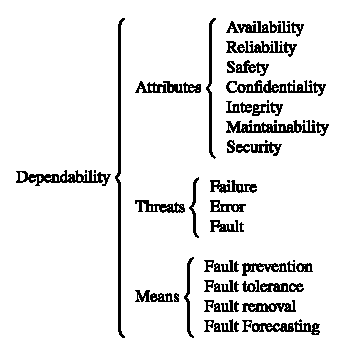
\includegraphics[width=0.33\textwidth]{imgs/div_avizienis}
    \caption{Dependability systematic classification.}
    \label{fig:div_avizienis}
\end{figure}

The first group is used to provide an analysis about the quality of a dependable
system. The second group brings the terms used to express undesirable threats --
but, in principle, not unexpected -- that makes a system become not dependable.
Finally, the third group shows the means and the techniques by which it becomes
possible to offer a dependable service.

About the second group, the term {\it failure} must be used to indicate when
a system behavior deviation occur, making it incapable to provide the service
for which was designed. An {\it error}, however, is related to the system state
and can lead to a failure. Briefly, if there is an error, then exists a sequence
of actions that can lead to a failure. Last, but not least, the term {\it fault}
is the cause of an error and is related to a defect. Normally, it is said that
the term fault may be defined as a defect that has the potential to generate
errors.

% ------------------------------------------------------------------------------
\subsection{Fault detection and diagnosis}
In order to ensure the success of planned operations and recognize the
behaviorial problems in the process, many supervision and monitoring systems are
being developed. According to \citet{chiang:2001}, among other functions, these
systems can detect, diagnose and eliminate faults, ensuring that the process
operations satisfies the performance specifications.

Additionally, the information provided by a monitoring system should not only
inform the system operator about what is going on, but also help him to take
corrective actions in order to remedy the problem. As a result, the ineffective
time will be reduced, the system protection will be increased and the
operational costs will be decreased.

\citet{chiang:2001} shows that there are four states involved in the process
monitoring: fault detection, fault isolation, fault diagnosis and fault
recovery, as shown in Fig. \ref{fig:states}. Although arranged as a sequence of
actions, all states are not always strictly necessary. Often, automated changes
from one state to another is transparent to the operator, displaying only the
crucial information to take appropriate action.

\begin{figure}[htb]
\centering
    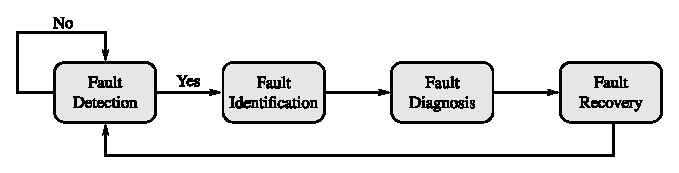
\includegraphics[width=0.6\textwidth]{imgs/states}
    \caption{States of fault detection and diagnosis.}
    \label{fig:states}
\end{figure}

% ==============================================================================
% PROPOSED SYSTEM
% ==============================================================================
\section{PROPOSED SYSTEM}\label{sec:proposed}
% ------------------------------------------------------------------------------
\subsection{Case study}
At the end of the introductory section, this paper proposes a system development
for FDD in a dynamic process. The process in question consists of a coupled
water tanks system developed by Quanser\reg, schematically represented in Fig.
\ref{fig:tanks}.

\begin{figure}[htb]
\centering
\subfigure[Original configuration.]
{
    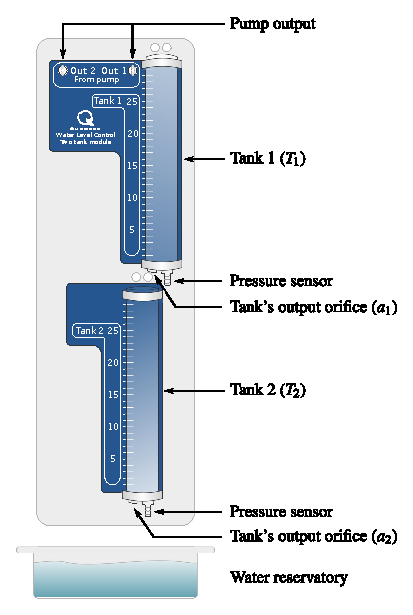
\includegraphics[height=245px]{imgs/tanks}
    \label{fig:tanks}
}
\qquad
\subfigure[Proposed configuration.]
{
    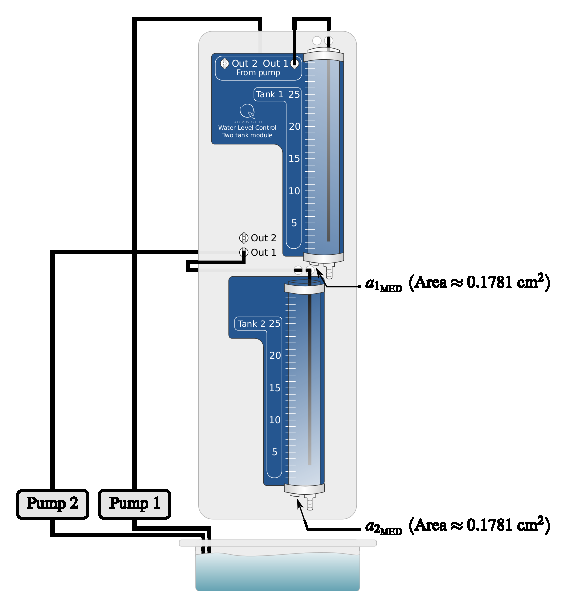
\includegraphics[height=245px]{imgs/new_config}
    \label{fig:new_config}
}
    \caption{Case study -- Coupled Water Tanks.}
\end{figure}

The tanks ($T_1$ e $T_2$) are mounted on the front of the support base and
positioned in such way that the water flows from the upper tank ($T_1$) to the
bottom tank ($T_2$) through orifice $a_1$, and from the $T_2$ to the water
reservatory through orifice $a_2$. The output water flow varies according to the
orifices $a_1$ and $a_2$, available in three different diameters.

Since the two tanks have the same cross-sectional area ($A_1 = A_2 = A$), their
dynamics are similar. However, find a mathematical model that adequately
describes the dynamics of such tanks is not so simple, because the general
equations of motion and energy that describe the fluid flow are quite
complicated. Therefore, some fundamental assumptions are needed. So, it is
assumed that the water in the tank is incompressible and the flow is
non-viscous, non-rotational and regular \citep{dorf:2009}. Considering these
aspects, after a series of algebraic manipulations using Bernoulli's equation,
the equations for a direct feed in $T_1$, can be described by Eqs.
(\ref{eq:l1_ponto}) and (\ref{eq:l2_ponto}).

\begin{eqnarray}
\dot{L_1} & = & \frac{K_m}{A}V_p -
                \left[\frac{a_1}{A}\sqrt{2g}\right]\sqrt{L_1}
                \label{eq:l1_ponto}\\
\dot{L_2} & = & \left[\frac{a_1}{A}\sqrt{2g}\right]\sqrt{L_1} -
                \left[\frac{a_2}{A}\sqrt{2g}\right]\sqrt{L_2}
                \label{eq:l2_ponto}
\end{eqnarray}
%
where $K_m$ represents the pump flow constant, $V_p$ the voltage applied to the
pump, $a_i$ the $T_i$'s output orifice, $L_i$ the water level in $T_i$ and $g$
the gravity acceleration.

In order to make the proposed system more generic and possibly make further
studies on fault tolerance, the system was modified by introducing another pump
with the same characteristics as the first one, as shown in Fig.
\ref{fig:new_config}. Clearly, in this case, the system has no longer a single
input and a single output (SISO). Now, the equations for the multiple input and
multiple output (MIMO) system can be described by Eqs. (\ref{eq:l1_ponto_fin})
and (\ref{eq:l2_ponto_fin}).

\begin{eqnarray}
\dot{L_1} & = & \frac{K_m}{A}V_{p_{\tiny 1}} -
                \left[\frac{a_1}{A}\sqrt{2g}\right]\sqrt{L_1}
                \label{eq:l1_ponto_fin}\\
\dot{L_2} & = & \frac{K_m}{A}V_{p_{\tiny 2}} +
                \left[\frac{a_1}{A}\sqrt{2g}\right]\sqrt{L_1} -
                \left[\frac{a_2}{A}\sqrt{2g}\right]\sqrt{L_2}
                \label{eq:l2_ponto_fin}
\end{eqnarray}
%
where $V_{p_{\tiny 1}}$ is the voltage applied to the first pump and
$V_{p_{\tiny 2}}$ is the voltage applied to the second pump.

% ------------------------------------------------------------------------------
\subsection{Simulated faults}
Despite the various faults that may exist in a coupled water tanks, only some of
these were selected to be simulated, as shown in Tab. \ref{tab:faults}.

\begin{table}[!htb]
\centering
\caption{Selected faults -- Classification.}
\label{tab:faults}
\begin{tabular}{|c|c|c|}
\hline
{\bf Fault \#} & {\bf Name} & {\bf Acronym}\\
\hline
\multicolumn{3}{|l|}{\bf Sensors}\\
\hline
1 & Uncalibrated Gain & UGSeF\\
\hline
2 & Uncalibrated Offset & UOSeF\\
\hline
3 & Noise Sensitivity & NSSeF\\
\hline
4 & Burned Sensor & BSeF\\
\hline
\multicolumn{3}{|l|}{\bf Actuators}\\
\hline
5 & Uncalibrated Gain & UGAF\\
\hline
6 & Uncalibrated Offset & UOAF\\
\hline
7 & Noise Sensitivity & NSAF\\
\hline
8 & $K_m$ variation & $K_m$AF\\
\hline
9 & Burned Actuator & BAF\\
\hline
\multicolumn{3}{|l|}{\bf Structural}\\
\hline
10 & Tank's Leak & TLStF\\
\hline
11 & Tank's $a_i$ variation & T$a_i$VStF\\
\hline
12 & Tank's $a_i$ obstruction & T$a_i$OStF\\
\hline
\end{tabular}
\end{table}

Since in these types of simulation the system is normally exposed to adverse
conditions, which could cause damage throughout the structure involved, the
proposed system was computationally simulated.

% ------------------------------------------------------------------------------
\subsection{Neural structures}
The neural networks for identification and FDD should be carefully chosen, since
an inappropriate choice can make the system innefective, not performing the
function for which it was assigned.

After a series of tests, the neural structure for identification, that must
represent the dynamics of the system, has a single neural network, which
receives as input the past values of the levels, $L_1(k-1)$ and $L_2 (k-1)$, and
voltages applied, $V_{p_{\tiny 1}} (k-1)$ and $V_{p_{\tiny 2}} (k-1)$,
generating, on its output, estimated levels, called $\widehat{L}_1 (k)$ and
$\widehat{L}_2 (k)$.  The best trained neural network for this purpose was
obtained from a second-order model NNARX with eight neurons on hidden layer. The
mean square error was $3.73 \times 10^{-6}$. The results obtained are not shown
because they are not the main focus of this paper.

The structure of FDD, in turn, was composed by twelve neural networks in which
each of these is associated with a single fault, configuring a set of
``specialists''. It is not, however, a committee machine, since there is no
network that performs the decision-making.

The input of each network is composed by the past values of the levels,
$L_1(k-1)$ and $L_2(k-1)$, the voltages applied to the pumps, $V_{p_{\tiny 1}}
(k-1)$ and $V_{p_{\tiny 2}} (k-1)$, and the residual errors produced from the
difference between the real and estimated output, $e_i (k) = L_i (k) -
\widehat{L}_i (k)$. The output of each network is a 2-bit binary word, which
indicates whether the fault is being detected in $T_1$, in $T_2$ or in $T_1$ and
$T_2$ simultaneously. A schematic diagram can be viewed in Fig.
\ref{fig:ann_fdd}.

\begin{figure}[htb]
\centering
    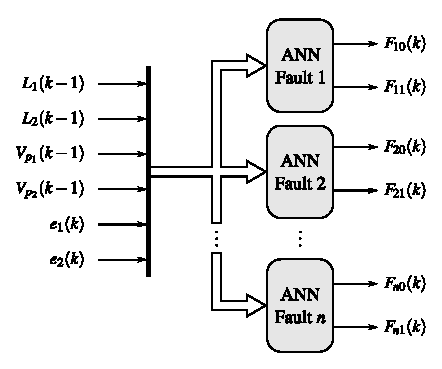
\includegraphics[width=0.4\textwidth]{imgs/ann_fdd}
    \caption{Neural network structure for fault detection and diagnosis.}
    \label{fig:ann_fdd}
\end{figure}

Opting for this disarticulated neural networks structure occurs by several
factors. An example that can be highlighted is the fact that more than one fault
may be happening simultaneously in the system. In this case, if only one neural
network was used, beyond the $N$ distinct words (one for each fault), the FDD
system should indicate each fault combination in the output. Considering only
the twelve selected faults, taken two by two, a total of 66 possible
combinations should to be generated. If all combinations were considered this
number would grow exorbitantly.

Moreover, a simple modification at one neural network will not affect in any
other. That is, if at any time is noticed that the introduction of a new
variable improves the detection for one fault, only one neural network needs to
be retrained. In future works, hibrid structures -- like neuro-fuzzy networks,
Kalman filters, statistical analysers and many more --, can be also utilized as
a specialist.

Once known all used subsystems, the proposed FDD system can be viewed in Fig.
\ref{fig:comp}. Attach this system to another, or associate it with a
Fault-Tolerant Control System (FTCS), can be made in a simple way, by processing
the information available at the output interface, named
\sequencia{F}{1}{2}{n}. However, this is not the objective here.

\begin{figure}[htb]
\centering
    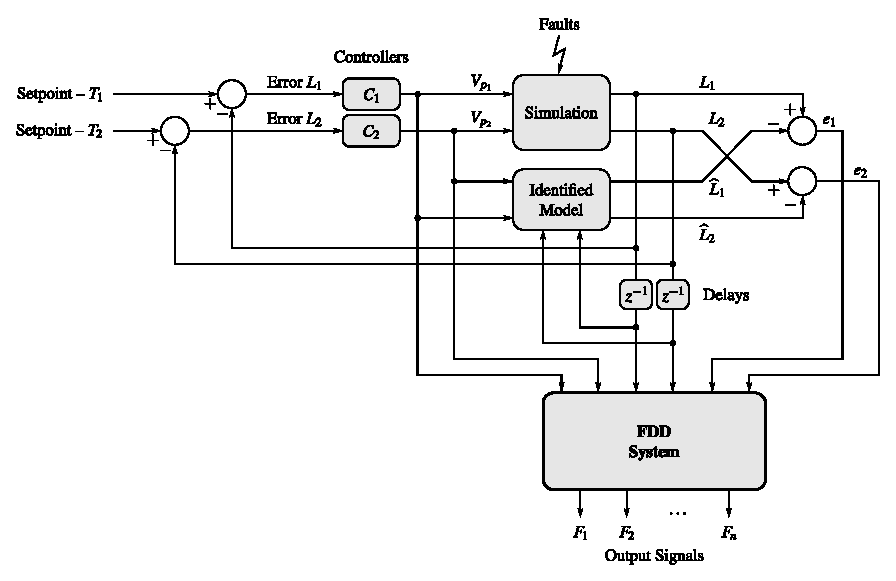
\includegraphics[width=0.8\textwidth]{imgs/comp}
    \caption{Proposed system schematic diagram.}
    \label{fig:comp}
\end{figure}

% ==============================================================================
% RESULTS
% ==============================================================================
\section{RESULTS}\label{sec:results}

% ------------------------------------------------------------------------------
\subsection{Data acquisition}
The first step to be taken for the identification and detection processes, is to
obtain the experimental samples for a supervised neural networks training. So,
the data acquisition was done by a stimulation of the simulated system through
the application of pseudo random binary signals (PRBSs) in the setpoint of each
tank and in the system fault parameters.

The range values applied to the setpoint varies between the minimum (zero) to
the maximum (thirty). For the fault detection, the values were applied as shown
in Tab. \ref{tab:values}. The values generated in the interval determined by the
minimum and maximum of each parameter were multiplied by the default values and
applied to the model.

\begin{table}[htb]
\caption{Applied values for training step.}
\label{tab:values}
\centering
\begin{threeparttable}
\begin{tabular}{|c|c|c|c|c|}
\hline
{\bf Fault} & {\bf Default value} & {\bf Min} & {\bf Max} & 
{\bf Representativeness}\\
\hline
UGSeF & 0,16\tnote{$*$} & 
0,8 & 1,2 & Up to $\pm$6\ cm\\
\hline
UOSeF & 1,0 & -3,0 & 3,0 & Up to $\pm$3\ cm\\
\hline
NSSeF & 1,0 & -0,03 & 0,03 & Up to $\pm$9\ cm\\
\hline
BSeF & 1,0 & 0,0 & 0,0 & -- \\
\hline
UGAF & 1,0 & 0,8 & 1,0 & Up to -3 Volts\\
\hline
UOAF & 1,0 & -1,0 & 0,0 & Up to -1 Volts\\
\hline
NSAF & 1,0 & -0,03 & 0,03 & Up to $\pm$0,45 Volts\\
\hline
$K_m$AF & $K_m$ & 0,7 & 1,1 & --\\
\hline
BAF & 1,0 & 0,0 & 0,0 & --\\
\hline
TLStF & $a_{i_{\text{\tiny MED}}}$\tnote{$**$} & 
0,25 & 0,75 & 25 a 75\% of $a_{i_{\text{\tiny MED}}}$\\
\hline
T$a_i$VStF & $a_{i_{\text{\tiny MED}}}$ & 
0,75 & 1,25 & $\pm$25\% of $a_{i_{\text{\tiny MED}}}$\\
\hline
T$a_i$OStF & $a_{i_{\text{\tiny MED}}}$ & 
0,0 & 0,5 & --\\
\hline
\end{tabular}
\begin{tablenotes}
\item [$*$] Established by the manufacturer.
\item [$**$] Cross-sectional area is approximately 0.1781\ cm${}^2$.
\end{tablenotes}
\end{threeparttable}
\end{table}

The PRBSs generated remains within the estabilished limits throughout the
simulation time. For the identification process were obtained 6000 (six
thousand) samples, equivalent to 10 (ten) minutes of simulation. For the
detection process, 20 (twenty) minutes was simulated, which corresponds to
12,000 (twelve thousand) samples. All data were collected with a sampling period
of 100 ms, identical to that used in the real process.

In possession of the obtained values, the neural networks training starts. All
networks were trained in offline mode with the neural networks toolbox of
Matlab\reg, using the LMA algorithm.

% ------------------------------------------------------------------------------
\subsection{Selected neural structures}
As already seen, the best network used for the model identification was obtained
from a second-order NNARX structure with eight neurons on hidden layer. This
network was selected among 54 others who had been trained for this same purpose
and has a mean square error of $3.73 \times 10^{-6}$.

For the FDD, the number of trained neural networks increases significantly. For
each order of the NNARX structure, the number of the neurons on hidden layer was
changed three times. Each time that number was changed, six neural networks were
trained, which guarantees that the selected networks would not be compromised by
convergence problems due the bad weights initialization or due to local minima.
Thus, for a second order structure, for example, were trained $3 \times 6 = 18$
neural networks.

The networks were selected from a second, third and fourth-order structures. So,
the number of trained networks would amount to $18 \times 3 = 54$ for each
fault. However, there were twelve faults to be trained. Thus, the total was $54
\times 12 = 648$ distinct neural networks.

Because of this large number, all the networks went through a validation process
with three simulations. In each simulation were recorded Type I and Type II
errors, composing an average error for each structure. The average values
obtained during the selection process can be viewed in Tab. \ref{tab:best_ann}.

\begin{table}[htb]
\centering
\caption{Best ANNs for FDD.}
\label{tab:best_ann}
\begin{threeparttable}
\begin{tabular}{|c|c|c|c|c|c|c|c|}
\hline
\multirow{2}{*}{\bf Fault} &
\multirow{2}{*}{\bf Order} &
\multirow{2}{*}{{\bf HLN}\tnote{$*$}} &
\multirow{2}{*}{\bf Train. \#} &
{\bf Correct} & {\bf Type I} & {\bf Type II} & {\bf Total}\\
& & & & {\bf Answers} & {\bf Errors} & {\bf Errors} & {\bf Errors (\%)}\\
\hline
UGSeF & 4 & 28 & 2 & 23491,33 & 203,33 & 305,33 & 2,12\%\\
\hline
UOSeF & 4 & 28 & 5 & 23890,33 & 8,66 & 101 & 0,46\%\\
\hline
NSSeF & 4 & 20 & 3 & 23317 & 324,66 & 358,33 & 2,84\%\\
\hline
BSeF & 4 & 20 & 4 & 23994 & 0,66 & 5,33 & 0,02\%\\
\hline
UGAF & 2 & 8 & 3 & 20710,33 & 1626,66 & 1663 & 13,7\%\\
\hline
UOAF & 4 & 28 & 3 & 23075,33 & 635,66 & 289 & 3,85\%\\
\hline
{NSAF} & 2 & 8 & 6 & 14153,33 & 3407 & 6439,66 & 41,03\%\\
\hline
$K_m$AF & 2 & 8 & 5 & 20764,66 & 1551,33 & 1684 & 13,48\%\\
\hline
BAF & 4 & 28 & 6 & 23980 & 2,33 & 17,66 & 0,083\%\\
\hline
TLStF & 4 & 24 & 1 & 23774,33 & 74 & 151,66 & 0,94\%\\
\hline
T$a_i$VStF & 2 & 8 & 3 & 22465,33 & 437 & 1097,66 & 6,39\%\\
\hline
T$a_i$OStF & 2 & 12 & 4 & 23995,66 & 1 & 3,33 & 0,018\%\\
\hline
\end{tabular}
\begin{tablenotes}
\item [$*$] Hidden layer neurons.
\end{tablenotes}
\end{threeparttable}
\end{table}

Having selected the best structures, the system was composed and submited to the
final simulation of one minute and forty five seconds, divided into intervals of
fifteen seconds as shown in Fig. \ref{fig:intervals}.

\begin{figure}[htb]
\centering
    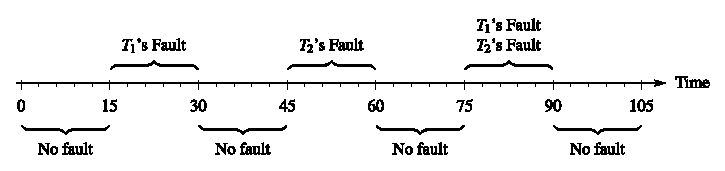
\includegraphics[width=0.7\textwidth]{imgs/intervals}
    \caption{Final simulation -- Intervals.}
    \label{fig:intervals}
\end{figure}

In this final test, the values of each fault parameter were kept fixed during
the interval in which that fault was acting in the system. The values of these
parameters are shown in Tab. \ref{tab:used_val}.

\begin{table}[htb]
\centering
\caption{Used parameter values.}
\label{tab:used_val}
\begin{tabular}{|c|c|c|}
\hline
{\bf Sim. \#} & {\bf Fault} & {\bf Modified value}\\
\hline
1 & UGSeF & $\text{Gain} = 0,128$\\
\hline
2 & UOSeF & -2,0\ cm\\
\hline
3 & NSSeF & $\pm$2\%\\
\hline
4 & BSeF & $\text{Gain} = 0,0$\\
\hline
5 & UGAF & $\text{Gain} = 0,8$\\
\hline
6 & UOAF & -0,5 Volts\\
\hline
7 & NSAF & $\pm$2\%\\
\hline
8 & $K_m$AF & $K_m = 3,45$\\ 
\hline
9 & BAF & $\text{Gain} = 0,0$\\
\hline
10 & TLStF & $a_{\text{\tiny VZ}} = a_{\text{\tiny MED}}/2$\\
\hline
11 & T$a_i$VStF & ${a_i}' = a_{\text{\tiny MED}}/2$\\
\hline
12 & T$a_i$OStF & ${a_i}' = a_{\text{\tiny MED}}/4$\\
\hline
\end{tabular}
\end{table}

% ------------------------------------------------------------------------------
\subsection{Obtained results}
The obtained results can be seen in Figs. \ref{fig:fsedg} to \ref{fig:fsivros}.
In these images, the red hatched areas represents the intervals in which the
fault was detected in $T_1$, while the blue hatched areas represents the
intervals in which the fault was detected in $T_2$.

The first fault to be simulated was UGSeF, whose the results can be seen in Fig.
\ref{fig:fsedg}. In this simulation the value of the sensor gain was reduced to
80\% of the default value.

\begin{figure}[htb]
    \begin{minipage}[b]{0.48\linewidth}
        \scalebox{0.65}{% GNUPLOT: LaTeX picture with Postscript
\begingroup
  \makeatletter
  \providecommand\color[2][]{%
    \GenericError{(gnuplot) \space\space\space\@spaces}{%
      Package color not loaded in conjunction with
      terminal option `colourtext'%
    }{See the gnuplot documentation for explanation.%
    }{Either use 'blacktext' in gnuplot or load the package
      color.sty in LaTeX.}%
    \renewcommand\color[2][]{}%
  }%
  \providecommand\includegraphics[2][]{%
    \GenericError{(gnuplot) \space\space\space\@spaces}{%
      Package graphicx or graphics not loaded%
    }{See the gnuplot documentation for explanation.%
    }{The gnuplot epslatex terminal needs graphicx.sty or graphics.sty.}%
    \renewcommand\includegraphics[2][]{}%
  }%
  \providecommand\rotatebox[2]{#2}%
  \@ifundefined{ifGPcolor}{%
    \newif\ifGPcolor
    \GPcolortrue
  }{}%
  \@ifundefined{ifGPblacktext}{%
    \newif\ifGPblacktext
    \GPblacktexttrue
  }{}%
  % define a \g@addto@macro without @ in the name:
  \let\gplgaddtomacro\g@addto@macro
  % define empty templates for all commands taking text:
  \gdef\gplbacktext{}%
  \gdef\gplfronttext{}%
  \makeatother
  \ifGPblacktext
    % no textcolor at all
    \def\colorrgb#1{}%
    \def\colorgray#1{}%
  \else
    % gray or color?
    \ifGPcolor
      \def\colorrgb#1{\color[rgb]{#1}}%
      \def\colorgray#1{\color[gray]{#1}}%
      \expandafter\def\csname LTw\endcsname{\color{white}}%
      \expandafter\def\csname LTb\endcsname{\color{black}}%
      \expandafter\def\csname LTa\endcsname{\color{black}}%
      \expandafter\def\csname LT0\endcsname{\color[rgb]{1,0,0}}%
      \expandafter\def\csname LT1\endcsname{\color[rgb]{0,1,0}}%
      \expandafter\def\csname LT2\endcsname{\color[rgb]{0,0,1}}%
      \expandafter\def\csname LT3\endcsname{\color[rgb]{1,0,1}}%
      \expandafter\def\csname LT4\endcsname{\color[rgb]{0,1,1}}%
      \expandafter\def\csname LT5\endcsname{\color[rgb]{1,1,0}}%
      \expandafter\def\csname LT6\endcsname{\color[rgb]{0,0,0}}%
      \expandafter\def\csname LT7\endcsname{\color[rgb]{1,0.3,0}}%
      \expandafter\def\csname LT8\endcsname{\color[rgb]{0.5,0.5,0.5}}%
    \else
      % gray
      \def\colorrgb#1{\color{black}}%
      \def\colorgray#1{\color[gray]{#1}}%
      \expandafter\def\csname LTw\endcsname{\color{white}}%
      \expandafter\def\csname LTb\endcsname{\color{black}}%
      \expandafter\def\csname LTa\endcsname{\color{black}}%
      \expandafter\def\csname LT0\endcsname{\color{black}}%
      \expandafter\def\csname LT1\endcsname{\color{black}}%
      \expandafter\def\csname LT2\endcsname{\color{black}}%
      \expandafter\def\csname LT3\endcsname{\color{black}}%
      \expandafter\def\csname LT4\endcsname{\color{black}}%
      \expandafter\def\csname LT5\endcsname{\color{black}}%
      \expandafter\def\csname LT6\endcsname{\color{black}}%
      \expandafter\def\csname LT7\endcsname{\color{black}}%
      \expandafter\def\csname LT8\endcsname{\color{black}}%
    \fi
  \fi
  \setlength{\unitlength}{0.0500bp}%
  \begin{picture}(7200.00,5040.00)%
    \gplgaddtomacro\gplbacktext{%
      \csname LTb\endcsname%
      \put(726,3150){\makebox(0,0)[r]{\strut{} 5}}%
      \csname LTb\endcsname%
      \put(726,3780){\makebox(0,0)[r]{\strut{} 10}}%
      \csname LTb\endcsname%
      \put(726,4409){\makebox(0,0)[r]{\strut{} 15}}%
      \csname LTb\endcsname%
      \put(726,5039){\makebox(0,0)[r]{\strut{} 20}}%
      \csname LTb\endcsname%
      \put(921,2237){\makebox(0,0){\strut{}}}%
      \csname LTb\endcsname%
      \put(1771,2237){\makebox(0,0){\strut{}}}%
      \csname LTb\endcsname%
      \put(2620,2237){\makebox(0,0){\strut{}}}%
      \csname LTb\endcsname%
      \put(3470,2237){\makebox(0,0){\strut{}}}%
      \csname LTb\endcsname%
      \put(4320,2237){\makebox(0,0){\strut{}}}%
      \csname LTb\endcsname%
      \put(5170,2237){\makebox(0,0){\strut{}}}%
      \csname LTb\endcsname%
      \put(6019,2237){\makebox(0,0){\strut{}}}%
      \csname LTb\endcsname%
      \put(6869,2237){\makebox(0,0){\strut{}}}%
      \put(352,3779){\rotatebox{-270}{\makebox(0,0){\strut{}Nível [cm]}}}%
    }%
    \gplgaddtomacro\gplfronttext{%
      \csname LTb\endcsname%
      \put(6278,2913){\makebox(0,0)[r]{\strut{}Ref. $T_1$}}%
      \csname LTb\endcsname%
      \put(6278,2693){\makebox(0,0)[r]{\strut{}Saída $T_1$}}%
    }%
    \gplgaddtomacro\gplbacktext{%
      \csname LTb\endcsname%
      \put(726,0){\makebox(0,0)[r]{\strut{} 0}}%
      \csname LTb\endcsname%
      \put(726,420){\makebox(0,0)[r]{\strut{} 5}}%
      \csname LTb\endcsname%
      \put(726,840){\makebox(0,0)[r]{\strut{} 10}}%
      \csname LTb\endcsname%
      \put(726,1260){\makebox(0,0)[r]{\strut{} 15}}%
      \csname LTb\endcsname%
      \put(726,1680){\makebox(0,0)[r]{\strut{} 20}}%
      \csname LTb\endcsname%
      \put(726,2100){\makebox(0,0)[r]{\strut{} 25}}%
      \csname LTb\endcsname%
      \put(726,2520){\makebox(0,0)[r]{\strut{} 30}}%
      \csname LTb\endcsname%
      \put(921,-283){\makebox(0,0){\strut{}0}}%
      \csname LTb\endcsname%
      \put(1771,-283){\makebox(0,0){\strut{}15}}%
      \csname LTb\endcsname%
      \put(2620,-283){\makebox(0,0){\strut{}30}}%
      \csname LTb\endcsname%
      \put(3470,-283){\makebox(0,0){\strut{}45}}%
      \csname LTb\endcsname%
      \put(4320,-283){\makebox(0,0){\strut{}60}}%
      \csname LTb\endcsname%
      \put(5170,-283){\makebox(0,0){\strut{}75}}%
      \csname LTb\endcsname%
      \put(6019,-283){\makebox(0,0){\strut{}90}}%
      \csname LTb\endcsname%
      \put(6869,-283){\makebox(0,0){\strut{}105}}%
      \put(352,1260){\rotatebox{-270}{\makebox(0,0){\strut{}Nível [cm]}}}%
      \put(3895,-613){\makebox(0,0){\strut{}Tempo [s]}}%
    }%
    \gplgaddtomacro\gplfronttext{%
      \csname LTb\endcsname%
      \put(6278,393){\makebox(0,0)[r]{\strut{}Ref. $T_2$}}%
      \csname LTb\endcsname%
      \put(6278,173){\makebox(0,0)[r]{\strut{}Saída $T_2$}}%
    }%
    \gplbacktext
    \put(0,0){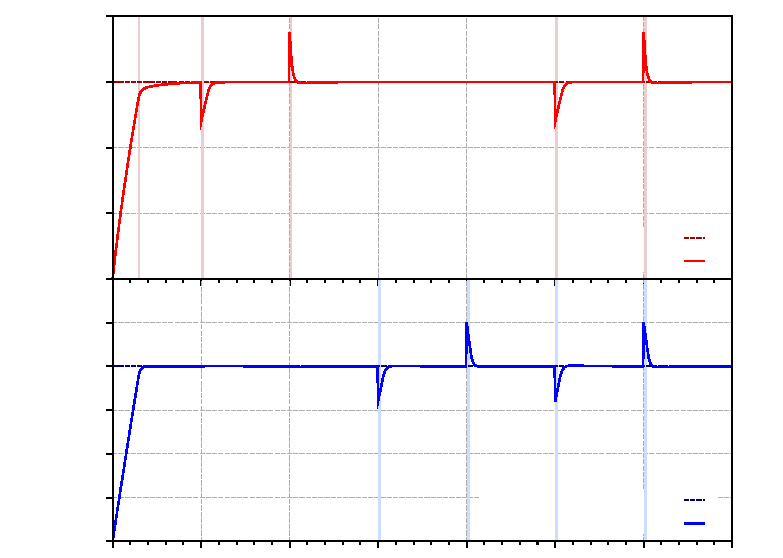
\includegraphics{fsedg}}%
    \gplfronttext
  \end{picture}%
\endgroup
}
        \vspace{0.5cm}
        \caption{UGSeF simulation -- Sensor's gain reduced to 80\% from the
                 default value.}
        \label{fig:fsedg}
    \end{minipage}
    \hfill
    \begin{minipage}[b]{0.48\linewidth}
        \scalebox{0.65}{% GNUPLOT: LaTeX picture with Postscript
\begingroup
  \makeatletter
  \providecommand\color[2][]{%
    \GenericError{(gnuplot) \space\space\space\@spaces}{%
      Package color not loaded in conjunction with
      terminal option `colourtext'%
    }{See the gnuplot documentation for explanation.%
    }{Either use 'blacktext' in gnuplot or load the package
      color.sty in LaTeX.}%
    \renewcommand\color[2][]{}%
  }%
  \providecommand\includegraphics[2][]{%
    \GenericError{(gnuplot) \space\space\space\@spaces}{%
      Package graphicx or graphics not loaded%
    }{See the gnuplot documentation for explanation.%
    }{The gnuplot epslatex terminal needs graphicx.sty or graphics.sty.}%
    \renewcommand\includegraphics[2][]{}%
  }%
  \providecommand\rotatebox[2]{#2}%
  \@ifundefined{ifGPcolor}{%
    \newif\ifGPcolor
    \GPcolortrue
  }{}%
  \@ifundefined{ifGPblacktext}{%
    \newif\ifGPblacktext
    \GPblacktexttrue
  }{}%
  % define a \g@addto@macro without @ in the name:
  \let\gplgaddtomacro\g@addto@macro
  % define empty templates for all commands taking text:
  \gdef\gplbacktext{}%
  \gdef\gplfronttext{}%
  \makeatother
  \ifGPblacktext
    % no textcolor at all
    \def\colorrgb#1{}%
    \def\colorgray#1{}%
  \else
    % gray or color?
    \ifGPcolor
      \def\colorrgb#1{\color[rgb]{#1}}%
      \def\colorgray#1{\color[gray]{#1}}%
      \expandafter\def\csname LTw\endcsname{\color{white}}%
      \expandafter\def\csname LTb\endcsname{\color{black}}%
      \expandafter\def\csname LTa\endcsname{\color{black}}%
      \expandafter\def\csname LT0\endcsname{\color[rgb]{1,0,0}}%
      \expandafter\def\csname LT1\endcsname{\color[rgb]{0,1,0}}%
      \expandafter\def\csname LT2\endcsname{\color[rgb]{0,0,1}}%
      \expandafter\def\csname LT3\endcsname{\color[rgb]{1,0,1}}%
      \expandafter\def\csname LT4\endcsname{\color[rgb]{0,1,1}}%
      \expandafter\def\csname LT5\endcsname{\color[rgb]{1,1,0}}%
      \expandafter\def\csname LT6\endcsname{\color[rgb]{0,0,0}}%
      \expandafter\def\csname LT7\endcsname{\color[rgb]{1,0.3,0}}%
      \expandafter\def\csname LT8\endcsname{\color[rgb]{0.5,0.5,0.5}}%
    \else
      % gray
      \def\colorrgb#1{\color{black}}%
      \def\colorgray#1{\color[gray]{#1}}%
      \expandafter\def\csname LTw\endcsname{\color{white}}%
      \expandafter\def\csname LTb\endcsname{\color{black}}%
      \expandafter\def\csname LTa\endcsname{\color{black}}%
      \expandafter\def\csname LT0\endcsname{\color{black}}%
      \expandafter\def\csname LT1\endcsname{\color{black}}%
      \expandafter\def\csname LT2\endcsname{\color{black}}%
      \expandafter\def\csname LT3\endcsname{\color{black}}%
      \expandafter\def\csname LT4\endcsname{\color{black}}%
      \expandafter\def\csname LT5\endcsname{\color{black}}%
      \expandafter\def\csname LT6\endcsname{\color{black}}%
      \expandafter\def\csname LT7\endcsname{\color{black}}%
      \expandafter\def\csname LT8\endcsname{\color{black}}%
    \fi
  \fi
  \setlength{\unitlength}{0.0500bp}%
  \begin{picture}(7200.00,5040.00)%
    \gplgaddtomacro\gplbacktext{%
      \csname LTb\endcsname%
      \put(726,3150){\makebox(0,0)[r]{\strut{} 5}}%
      \csname LTb\endcsname%
      \put(726,3780){\makebox(0,0)[r]{\strut{} 10}}%
      \csname LTb\endcsname%
      \put(726,4409){\makebox(0,0)[r]{\strut{} 15}}%
      \csname LTb\endcsname%
      \put(726,5039){\makebox(0,0)[r]{\strut{} 20}}%
      \csname LTb\endcsname%
      \put(921,2237){\makebox(0,0){\strut{}}}%
      \csname LTb\endcsname%
      \put(1771,2237){\makebox(0,0){\strut{}}}%
      \csname LTb\endcsname%
      \put(2620,2237){\makebox(0,0){\strut{}}}%
      \csname LTb\endcsname%
      \put(3470,2237){\makebox(0,0){\strut{}}}%
      \csname LTb\endcsname%
      \put(4320,2237){\makebox(0,0){\strut{}}}%
      \csname LTb\endcsname%
      \put(5170,2237){\makebox(0,0){\strut{}}}%
      \csname LTb\endcsname%
      \put(6019,2237){\makebox(0,0){\strut{}}}%
      \csname LTb\endcsname%
      \put(6869,2237){\makebox(0,0){\strut{}}}%
      \put(352,3779){\rotatebox{-270}{\makebox(0,0){\strut{}Level [cm]}}}%
    }%
    \gplgaddtomacro\gplfronttext{%
      \csname LTb\endcsname%
      \put(6278,2913){\makebox(0,0)[r]{\strut{}Setpoint $T_1$}}%
      \csname LTb\endcsname%
      \put(6278,2693){\makebox(0,0)[r]{\strut{}Output $T_1$}}%
    }%
    \gplgaddtomacro\gplbacktext{%
      \csname LTb\endcsname%
      \put(726,0){\makebox(0,0)[r]{\strut{} 0}}%
      \csname LTb\endcsname%
      \put(726,504){\makebox(0,0)[r]{\strut{} 5}}%
      \csname LTb\endcsname%
      \put(726,1008){\makebox(0,0)[r]{\strut{} 10}}%
      \csname LTb\endcsname%
      \put(726,1512){\makebox(0,0)[r]{\strut{} 15}}%
      \csname LTb\endcsname%
      \put(726,2016){\makebox(0,0)[r]{\strut{} 20}}%
      \csname LTb\endcsname%
      \put(726,2520){\makebox(0,0)[r]{\strut{} 25}}%
      \csname LTb\endcsname%
      \put(921,-283){\makebox(0,0){\strut{}0}}%
      \csname LTb\endcsname%
      \put(1771,-283){\makebox(0,0){\strut{}15}}%
      \csname LTb\endcsname%
      \put(2620,-283){\makebox(0,0){\strut{}30}}%
      \csname LTb\endcsname%
      \put(3470,-283){\makebox(0,0){\strut{}45}}%
      \csname LTb\endcsname%
      \put(4320,-283){\makebox(0,0){\strut{}60}}%
      \csname LTb\endcsname%
      \put(5170,-283){\makebox(0,0){\strut{}75}}%
      \csname LTb\endcsname%
      \put(6019,-283){\makebox(0,0){\strut{}90}}%
      \csname LTb\endcsname%
      \put(6869,-283){\makebox(0,0){\strut{}105}}%
      \put(352,1260){\rotatebox{-270}{\makebox(0,0){\strut{}Level [cm]}}}%
      \put(3895,-613){\makebox(0,0){\strut{}Time [s]}}%
    }%
    \gplgaddtomacro\gplfronttext{%
      \csname LTb\endcsname%
      \put(6278,393){\makebox(0,0)[r]{\strut{}Setpoint $T_2$}}%
      \csname LTb\endcsname%
      \put(6278,173){\makebox(0,0)[r]{\strut{}Output $T_2$}}%
    }%
    \gplbacktext
    \put(0,0){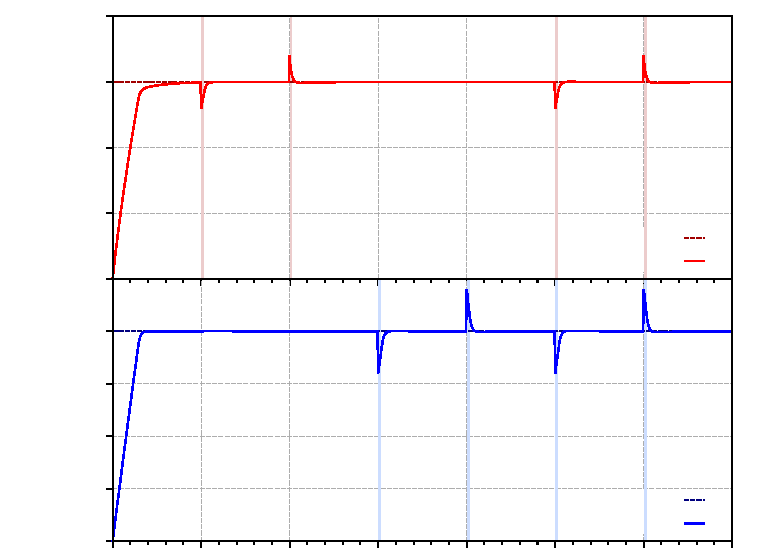
\includegraphics{fsedo}}%
    \gplfronttext
  \end{picture}%
\endgroup
}
        \vspace{0.5cm}
        \caption{UOSeF simulation -- Sensor's offset configured to $-2$ cm.}
        \label{fig:fsedo}
    \end{minipage}
\end{figure}

\begin{figure}[htb]
    \begin{minipage}[b]{0.48\linewidth}
        \scalebox{0.65}{% GNUPLOT: LaTeX picture with Postscript
\begingroup
  \makeatletter
  \providecommand\color[2][]{%
    \GenericError{(gnuplot) \space\space\space\@spaces}{%
      Package color not loaded in conjunction with
      terminal option `colourtext'%
    }{See the gnuplot documentation for explanation.%
    }{Either use 'blacktext' in gnuplot or load the package
      color.sty in LaTeX.}%
    \renewcommand\color[2][]{}%
  }%
  \providecommand\includegraphics[2][]{%
    \GenericError{(gnuplot) \space\space\space\@spaces}{%
      Package graphicx or graphics not loaded%
    }{See the gnuplot documentation for explanation.%
    }{The gnuplot epslatex terminal needs graphicx.sty or graphics.sty.}%
    \renewcommand\includegraphics[2][]{}%
  }%
  \providecommand\rotatebox[2]{#2}%
  \@ifundefined{ifGPcolor}{%
    \newif\ifGPcolor
    \GPcolortrue
  }{}%
  \@ifundefined{ifGPblacktext}{%
    \newif\ifGPblacktext
    \GPblacktexttrue
  }{}%
  % define a \g@addto@macro without @ in the name:
  \let\gplgaddtomacro\g@addto@macro
  % define empty templates for all commands taking text:
  \gdef\gplbacktext{}%
  \gdef\gplfronttext{}%
  \makeatother
  \ifGPblacktext
    % no textcolor at all
    \def\colorrgb#1{}%
    \def\colorgray#1{}%
  \else
    % gray or color?
    \ifGPcolor
      \def\colorrgb#1{\color[rgb]{#1}}%
      \def\colorgray#1{\color[gray]{#1}}%
      \expandafter\def\csname LTw\endcsname{\color{white}}%
      \expandafter\def\csname LTb\endcsname{\color{black}}%
      \expandafter\def\csname LTa\endcsname{\color{black}}%
      \expandafter\def\csname LT0\endcsname{\color[rgb]{1,0,0}}%
      \expandafter\def\csname LT1\endcsname{\color[rgb]{0,1,0}}%
      \expandafter\def\csname LT2\endcsname{\color[rgb]{0,0,1}}%
      \expandafter\def\csname LT3\endcsname{\color[rgb]{1,0,1}}%
      \expandafter\def\csname LT4\endcsname{\color[rgb]{0,1,1}}%
      \expandafter\def\csname LT5\endcsname{\color[rgb]{1,1,0}}%
      \expandafter\def\csname LT6\endcsname{\color[rgb]{0,0,0}}%
      \expandafter\def\csname LT7\endcsname{\color[rgb]{1,0.3,0}}%
      \expandafter\def\csname LT8\endcsname{\color[rgb]{0.5,0.5,0.5}}%
    \else
      % gray
      \def\colorrgb#1{\color{black}}%
      \def\colorgray#1{\color[gray]{#1}}%
      \expandafter\def\csname LTw\endcsname{\color{white}}%
      \expandafter\def\csname LTb\endcsname{\color{black}}%
      \expandafter\def\csname LTa\endcsname{\color{black}}%
      \expandafter\def\csname LT0\endcsname{\color{black}}%
      \expandafter\def\csname LT1\endcsname{\color{black}}%
      \expandafter\def\csname LT2\endcsname{\color{black}}%
      \expandafter\def\csname LT3\endcsname{\color{black}}%
      \expandafter\def\csname LT4\endcsname{\color{black}}%
      \expandafter\def\csname LT5\endcsname{\color{black}}%
      \expandafter\def\csname LT6\endcsname{\color{black}}%
      \expandafter\def\csname LT7\endcsname{\color{black}}%
      \expandafter\def\csname LT8\endcsname{\color{black}}%
    \fi
  \fi
  \setlength{\unitlength}{0.0500bp}%
  \begin{picture}(7200.00,5040.00)%
    \gplgaddtomacro\gplbacktext{%
      \csname LTb\endcsname%
      \put(726,3150){\makebox(0,0)[r]{\strut{} 5}}%
      \csname LTb\endcsname%
      \put(726,3780){\makebox(0,0)[r]{\strut{} 10}}%
      \csname LTb\endcsname%
      \put(726,4409){\makebox(0,0)[r]{\strut{} 15}}%
      \csname LTb\endcsname%
      \put(726,5039){\makebox(0,0)[r]{\strut{} 20}}%
      \csname LTb\endcsname%
      \put(921,2237){\makebox(0,0){\strut{}}}%
      \csname LTb\endcsname%
      \put(1771,2237){\makebox(0,0){\strut{}}}%
      \csname LTb\endcsname%
      \put(2620,2237){\makebox(0,0){\strut{}}}%
      \csname LTb\endcsname%
      \put(3470,2237){\makebox(0,0){\strut{}}}%
      \csname LTb\endcsname%
      \put(4320,2237){\makebox(0,0){\strut{}}}%
      \csname LTb\endcsname%
      \put(5170,2237){\makebox(0,0){\strut{}}}%
      \csname LTb\endcsname%
      \put(6019,2237){\makebox(0,0){\strut{}}}%
      \csname LTb\endcsname%
      \put(6869,2237){\makebox(0,0){\strut{}}}%
      \put(352,3779){\rotatebox{-270}{\makebox(0,0){\strut{}Nível [cm]}}}%
    }%
    \gplgaddtomacro\gplfronttext{%
      \csname LTb\endcsname%
      \put(6278,2913){\makebox(0,0)[r]{\strut{}Ref. $T_1$}}%
      \csname LTb\endcsname%
      \put(6278,2693){\makebox(0,0)[r]{\strut{}Saída $T_1$}}%
    }%
    \gplgaddtomacro\gplbacktext{%
      \csname LTb\endcsname%
      \put(726,0){\makebox(0,0)[r]{\strut{} 0}}%
      \csname LTb\endcsname%
      \put(726,840){\makebox(0,0)[r]{\strut{} 10}}%
      \csname LTb\endcsname%
      \put(726,1680){\makebox(0,0)[r]{\strut{} 20}}%
      \csname LTb\endcsname%
      \put(726,2520){\makebox(0,0)[r]{\strut{} 30}}%
      \csname LTb\endcsname%
      \put(921,-283){\makebox(0,0){\strut{}0}}%
      \csname LTb\endcsname%
      \put(1771,-283){\makebox(0,0){\strut{}15}}%
      \csname LTb\endcsname%
      \put(2620,-283){\makebox(0,0){\strut{}30}}%
      \csname LTb\endcsname%
      \put(3470,-283){\makebox(0,0){\strut{}45}}%
      \csname LTb\endcsname%
      \put(4320,-283){\makebox(0,0){\strut{}60}}%
      \csname LTb\endcsname%
      \put(5170,-283){\makebox(0,0){\strut{}75}}%
      \csname LTb\endcsname%
      \put(6019,-283){\makebox(0,0){\strut{}90}}%
      \csname LTb\endcsname%
      \put(6869,-283){\makebox(0,0){\strut{}105}}%
      \put(352,1260){\rotatebox{-270}{\makebox(0,0){\strut{}Nível [cm]}}}%
      \put(3895,-613){\makebox(0,0){\strut{}Tempo [s]}}%
    }%
    \gplgaddtomacro\gplfronttext{%
      \csname LTb\endcsname%
      \put(6278,393){\makebox(0,0)[r]{\strut{}Ref. $T_2$}}%
      \csname LTb\endcsname%
      \put(6278,173){\makebox(0,0)[r]{\strut{}Saída $T_2$}}%
    }%
    \gplbacktext
    \put(0,0){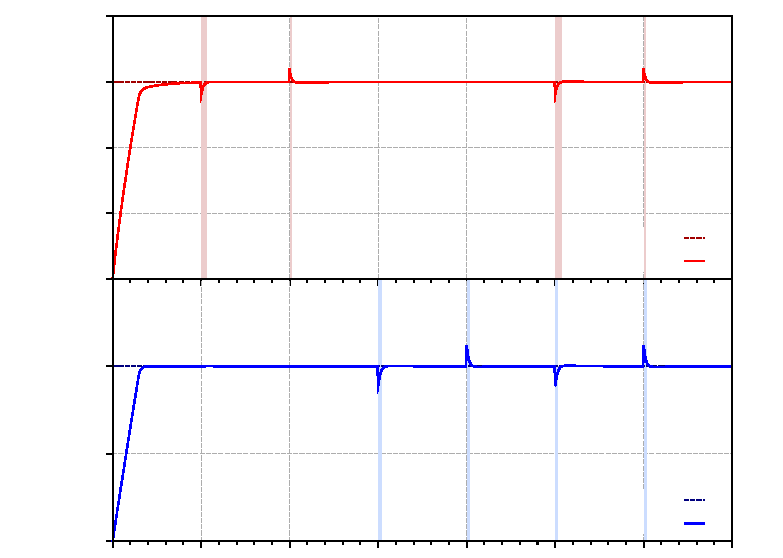
\includegraphics{fsivzt}}%
    \gplfronttext
  \end{picture}%
\endgroup
}
        \vspace{0.5cm}
        \caption{TLStF simulation -- Where $a_{\tiny L} = a_{\tiny
                 \text{MED}}/2$ and $a_{\tiny \text{MED}} \approx 0.1781$
                 cm\textsuperscript{2}.}
        \label{fig:fsivzt}
    \end{minipage}
    \hfill
    \begin{minipage}[b]{0.48\linewidth}
        \scalebox{0.65}{% GNUPLOT: LaTeX picture with Postscript
\begingroup
  \makeatletter
  \providecommand\color[2][]{%
    \GenericError{(gnuplot) \space\space\space\@spaces}{%
      Package color not loaded in conjunction with
      terminal option `colourtext'%
    }{See the gnuplot documentation for explanation.%
    }{Either use 'blacktext' in gnuplot or load the package
      color.sty in LaTeX.}%
    \renewcommand\color[2][]{}%
  }%
  \providecommand\includegraphics[2][]{%
    \GenericError{(gnuplot) \space\space\space\@spaces}{%
      Package graphicx or graphics not loaded%
    }{See the gnuplot documentation for explanation.%
    }{The gnuplot epslatex terminal needs graphicx.sty or graphics.sty.}%
    \renewcommand\includegraphics[2][]{}%
  }%
  \providecommand\rotatebox[2]{#2}%
  \@ifundefined{ifGPcolor}{%
    \newif\ifGPcolor
    \GPcolortrue
  }{}%
  \@ifundefined{ifGPblacktext}{%
    \newif\ifGPblacktext
    \GPblacktexttrue
  }{}%
  % define a \g@addto@macro without @ in the name:
  \let\gplgaddtomacro\g@addto@macro
  % define empty templates for all commands taking text:
  \gdef\gplbacktext{}%
  \gdef\gplfronttext{}%
  \makeatother
  \ifGPblacktext
    % no textcolor at all
    \def\colorrgb#1{}%
    \def\colorgray#1{}%
  \else
    % gray or color?
    \ifGPcolor
      \def\colorrgb#1{\color[rgb]{#1}}%
      \def\colorgray#1{\color[gray]{#1}}%
      \expandafter\def\csname LTw\endcsname{\color{white}}%
      \expandafter\def\csname LTb\endcsname{\color{black}}%
      \expandafter\def\csname LTa\endcsname{\color{black}}%
      \expandafter\def\csname LT0\endcsname{\color[rgb]{1,0,0}}%
      \expandafter\def\csname LT1\endcsname{\color[rgb]{0,1,0}}%
      \expandafter\def\csname LT2\endcsname{\color[rgb]{0,0,1}}%
      \expandafter\def\csname LT3\endcsname{\color[rgb]{1,0,1}}%
      \expandafter\def\csname LT4\endcsname{\color[rgb]{0,1,1}}%
      \expandafter\def\csname LT5\endcsname{\color[rgb]{1,1,0}}%
      \expandafter\def\csname LT6\endcsname{\color[rgb]{0,0,0}}%
      \expandafter\def\csname LT7\endcsname{\color[rgb]{1,0.3,0}}%
      \expandafter\def\csname LT8\endcsname{\color[rgb]{0.5,0.5,0.5}}%
    \else
      % gray
      \def\colorrgb#1{\color{black}}%
      \def\colorgray#1{\color[gray]{#1}}%
      \expandafter\def\csname LTw\endcsname{\color{white}}%
      \expandafter\def\csname LTb\endcsname{\color{black}}%
      \expandafter\def\csname LTa\endcsname{\color{black}}%
      \expandafter\def\csname LT0\endcsname{\color{black}}%
      \expandafter\def\csname LT1\endcsname{\color{black}}%
      \expandafter\def\csname LT2\endcsname{\color{black}}%
      \expandafter\def\csname LT3\endcsname{\color{black}}%
      \expandafter\def\csname LT4\endcsname{\color{black}}%
      \expandafter\def\csname LT5\endcsname{\color{black}}%
      \expandafter\def\csname LT6\endcsname{\color{black}}%
      \expandafter\def\csname LT7\endcsname{\color{black}}%
      \expandafter\def\csname LT8\endcsname{\color{black}}%
    \fi
  \fi
  \setlength{\unitlength}{0.0500bp}%
  \begin{picture}(7200.00,5040.00)%
    \gplgaddtomacro\gplbacktext{%
      \csname LTb\endcsname%
      \put(726,3150){\makebox(0,0)[r]{\strut{} 5}}%
      \csname LTb\endcsname%
      \put(726,3780){\makebox(0,0)[r]{\strut{} 10}}%
      \csname LTb\endcsname%
      \put(726,4409){\makebox(0,0)[r]{\strut{} 15}}%
      \csname LTb\endcsname%
      \put(726,5039){\makebox(0,0)[r]{\strut{} 20}}%
      \csname LTb\endcsname%
      \put(921,2237){\makebox(0,0){\strut{}}}%
      \csname LTb\endcsname%
      \put(1771,2237){\makebox(0,0){\strut{}}}%
      \csname LTb\endcsname%
      \put(2620,2237){\makebox(0,0){\strut{}}}%
      \csname LTb\endcsname%
      \put(3470,2237){\makebox(0,0){\strut{}}}%
      \csname LTb\endcsname%
      \put(4320,2237){\makebox(0,0){\strut{}}}%
      \csname LTb\endcsname%
      \put(5170,2237){\makebox(0,0){\strut{}}}%
      \csname LTb\endcsname%
      \put(6019,2237){\makebox(0,0){\strut{}}}%
      \csname LTb\endcsname%
      \put(6869,2237){\makebox(0,0){\strut{}}}%
      \put(352,3779){\rotatebox{-270}{\makebox(0,0){\strut{}Nível [cm]}}}%
    }%
    \gplgaddtomacro\gplfronttext{%
      \csname LTb\endcsname%
      \put(6278,2913){\makebox(0,0)[r]{\strut{}Ref. $T_1$}}%
      \csname LTb\endcsname%
      \put(6278,2693){\makebox(0,0)[r]{\strut{}Saída $T_1$}}%
    }%
    \gplgaddtomacro\gplbacktext{%
      \csname LTb\endcsname%
      \put(726,0){\makebox(0,0)[r]{\strut{} 0}}%
      \csname LTb\endcsname%
      \put(726,504){\makebox(0,0)[r]{\strut{} 5}}%
      \csname LTb\endcsname%
      \put(726,1008){\makebox(0,0)[r]{\strut{} 10}}%
      \csname LTb\endcsname%
      \put(726,1512){\makebox(0,0)[r]{\strut{} 15}}%
      \csname LTb\endcsname%
      \put(726,2016){\makebox(0,0)[r]{\strut{} 20}}%
      \csname LTb\endcsname%
      \put(726,2520){\makebox(0,0)[r]{\strut{} 25}}%
      \csname LTb\endcsname%
      \put(921,-283){\makebox(0,0){\strut{}0}}%
      \csname LTb\endcsname%
      \put(1771,-283){\makebox(0,0){\strut{}15}}%
      \csname LTb\endcsname%
      \put(2620,-283){\makebox(0,0){\strut{}30}}%
      \csname LTb\endcsname%
      \put(3470,-283){\makebox(0,0){\strut{}45}}%
      \csname LTb\endcsname%
      \put(4320,-283){\makebox(0,0){\strut{}60}}%
      \csname LTb\endcsname%
      \put(5170,-283){\makebox(0,0){\strut{}75}}%
      \csname LTb\endcsname%
      \put(6019,-283){\makebox(0,0){\strut{}90}}%
      \csname LTb\endcsname%
      \put(6869,-283){\makebox(0,0){\strut{}105}}%
      \put(352,1260){\rotatebox{-270}{\makebox(0,0){\strut{}Nível [cm]}}}%
      \put(3895,-613){\makebox(0,0){\strut{}Tempo [s]}}%
    }%
    \gplgaddtomacro\gplfronttext{%
      \csname LTb\endcsname%
      \put(6278,393){\makebox(0,0)[r]{\strut{}Ref. $T_2$}}%
      \csname LTb\endcsname%
      \put(6278,173){\makebox(0,0)[r]{\strut{}Saída $T_2$}}%
    }%
    \gplbacktext
    \put(0,0){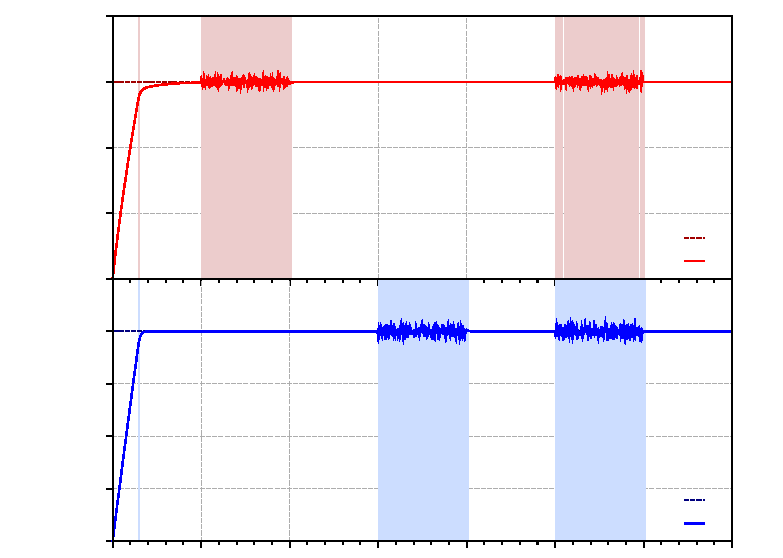
\includegraphics{fsesr}}%
    \gplfronttext
  \end{picture}%
\endgroup
}
        \vspace{0.5cm}
        \caption{NSSeF simulation -- Assumming a uniform distribution noise from
                 $\pm$2\%.}
        \label{fig:fsesr}
    \end{minipage}
\end{figure}

In this figure, the system can identify the presence of the fault only when the
parameter value is modified. After this period, the controllers can
``compensate'' the fault, sending more voltage to the pump and thus causing the
return to the setpoint. However, that ``compensation'' is done improperly, given
that the reading has an error of 20\%.

Thus, when the value read by the sensors is 24 cm, the tank is about to
overflow, reaching, in fact, the upper limit of 30 cm. In an academic
application this may not represent any risk to equipments beyond those in which
the water could cause. But, in critical applications, that ``compensation''
may bring several damages.

The system behaved in a similar manner to that in UOSeF and TLStF, as observed
in Figs. \ref{fig:fsedo} and \ref{fig:fsivzt}. Especially for the TLStF
simulation, is considered another output orifice, named $a_{\tiny L}$, that has
the same characteristics of the tank output orifice $a_i$, but different
diameter.

The results for these faults are not consistent with the Tab.
\ref{tab:best_ann}. This situation may be ocurring because the networks has
identified the rapid dynamic changes of the PRBS, failing to identify continuous
abrupt changes.

A possible alternative to solve this problem would be to use binary flags,
activated at the time that the first variation was detected and deactivated in
the next detection. These flags indicate that the faults are acting during the
time interval in which they were active.

Another simulation shows that the NSSeF was easily identified by the system, as
shown in Fig. \ref{fig:fsesr}. However, due to the noise with uniform
distribution ($\pm$2\%), the system can not detect the fault at some points. At
these points, the value generated by the {\tt rand} function keeps the signal
next to the setpoint.

\begin{figure}[htb]
    \begin{minipage}[b]{0.48\linewidth}
        \scalebox{0.65}{% GNUPLOT: LaTeX picture with Postscript
\begingroup
  \makeatletter
  \providecommand\color[2][]{%
    \GenericError{(gnuplot) \space\space\space\@spaces}{%
      Package color not loaded in conjunction with
      terminal option `colourtext'%
    }{See the gnuplot documentation for explanation.%
    }{Either use 'blacktext' in gnuplot or load the package
      color.sty in LaTeX.}%
    \renewcommand\color[2][]{}%
  }%
  \providecommand\includegraphics[2][]{%
    \GenericError{(gnuplot) \space\space\space\@spaces}{%
      Package graphicx or graphics not loaded%
    }{See the gnuplot documentation for explanation.%
    }{The gnuplot epslatex terminal needs graphicx.sty or graphics.sty.}%
    \renewcommand\includegraphics[2][]{}%
  }%
  \providecommand\rotatebox[2]{#2}%
  \@ifundefined{ifGPcolor}{%
    \newif\ifGPcolor
    \GPcolortrue
  }{}%
  \@ifundefined{ifGPblacktext}{%
    \newif\ifGPblacktext
    \GPblacktexttrue
  }{}%
  % define a \g@addto@macro without @ in the name:
  \let\gplgaddtomacro\g@addto@macro
  % define empty templates for all commands taking text:
  \gdef\gplbacktext{}%
  \gdef\gplfronttext{}%
  \makeatother
  \ifGPblacktext
    % no textcolor at all
    \def\colorrgb#1{}%
    \def\colorgray#1{}%
  \else
    % gray or color?
    \ifGPcolor
      \def\colorrgb#1{\color[rgb]{#1}}%
      \def\colorgray#1{\color[gray]{#1}}%
      \expandafter\def\csname LTw\endcsname{\color{white}}%
      \expandafter\def\csname LTb\endcsname{\color{black}}%
      \expandafter\def\csname LTa\endcsname{\color{black}}%
      \expandafter\def\csname LT0\endcsname{\color[rgb]{1,0,0}}%
      \expandafter\def\csname LT1\endcsname{\color[rgb]{0,1,0}}%
      \expandafter\def\csname LT2\endcsname{\color[rgb]{0,0,1}}%
      \expandafter\def\csname LT3\endcsname{\color[rgb]{1,0,1}}%
      \expandafter\def\csname LT4\endcsname{\color[rgb]{0,1,1}}%
      \expandafter\def\csname LT5\endcsname{\color[rgb]{1,1,0}}%
      \expandafter\def\csname LT6\endcsname{\color[rgb]{0,0,0}}%
      \expandafter\def\csname LT7\endcsname{\color[rgb]{1,0.3,0}}%
      \expandafter\def\csname LT8\endcsname{\color[rgb]{0.5,0.5,0.5}}%
    \else
      % gray
      \def\colorrgb#1{\color{black}}%
      \def\colorgray#1{\color[gray]{#1}}%
      \expandafter\def\csname LTw\endcsname{\color{white}}%
      \expandafter\def\csname LTb\endcsname{\color{black}}%
      \expandafter\def\csname LTa\endcsname{\color{black}}%
      \expandafter\def\csname LT0\endcsname{\color{black}}%
      \expandafter\def\csname LT1\endcsname{\color{black}}%
      \expandafter\def\csname LT2\endcsname{\color{black}}%
      \expandafter\def\csname LT3\endcsname{\color{black}}%
      \expandafter\def\csname LT4\endcsname{\color{black}}%
      \expandafter\def\csname LT5\endcsname{\color{black}}%
      \expandafter\def\csname LT6\endcsname{\color{black}}%
      \expandafter\def\csname LT7\endcsname{\color{black}}%
      \expandafter\def\csname LT8\endcsname{\color{black}}%
    \fi
  \fi
  \setlength{\unitlength}{0.0500bp}%
  \begin{picture}(7200.00,5040.00)%
    \gplgaddtomacro\gplbacktext{%
      \csname LTb\endcsname%
      \put(726,3150){\makebox(0,0)[r]{\strut{} 5}}%
      \csname LTb\endcsname%
      \put(726,3780){\makebox(0,0)[r]{\strut{} 10}}%
      \csname LTb\endcsname%
      \put(726,4409){\makebox(0,0)[r]{\strut{} 15}}%
      \csname LTb\endcsname%
      \put(726,5039){\makebox(0,0)[r]{\strut{} 20}}%
      \csname LTb\endcsname%
      \put(921,2237){\makebox(0,0){\strut{}}}%
      \csname LTb\endcsname%
      \put(1771,2237){\makebox(0,0){\strut{}}}%
      \csname LTb\endcsname%
      \put(2620,2237){\makebox(0,0){\strut{}}}%
      \csname LTb\endcsname%
      \put(3470,2237){\makebox(0,0){\strut{}}}%
      \csname LTb\endcsname%
      \put(4320,2237){\makebox(0,0){\strut{}}}%
      \csname LTb\endcsname%
      \put(5170,2237){\makebox(0,0){\strut{}}}%
      \csname LTb\endcsname%
      \put(6019,2237){\makebox(0,0){\strut{}}}%
      \csname LTb\endcsname%
      \put(6869,2237){\makebox(0,0){\strut{}}}%
      \put(352,3779){\rotatebox{-270}{\makebox(0,0){\strut{}Level [cm]}}}%
    }%
    \gplgaddtomacro\gplfronttext{%
      \csname LTb\endcsname%
      \put(6278,2913){\makebox(0,0)[r]{\strut{}Setpoint $T_1$}}%
      \csname LTb\endcsname%
      \put(6278,2693){\makebox(0,0)[r]{\strut{}Output $T_1$}}%
    }%
    \gplgaddtomacro\gplbacktext{%
      \csname LTb\endcsname%
      \put(726,0){\makebox(0,0)[r]{\strut{} 0}}%
      \csname LTb\endcsname%
      \put(726,840){\makebox(0,0)[r]{\strut{} 10}}%
      \csname LTb\endcsname%
      \put(726,1680){\makebox(0,0)[r]{\strut{} 20}}%
      \csname LTb\endcsname%
      \put(726,2520){\makebox(0,0)[r]{\strut{} 30}}%
      \csname LTb\endcsname%
      \put(921,-283){\makebox(0,0){\strut{}0}}%
      \csname LTb\endcsname%
      \put(1771,-283){\makebox(0,0){\strut{}15}}%
      \csname LTb\endcsname%
      \put(2620,-283){\makebox(0,0){\strut{}30}}%
      \csname LTb\endcsname%
      \put(3470,-283){\makebox(0,0){\strut{}45}}%
      \csname LTb\endcsname%
      \put(4320,-283){\makebox(0,0){\strut{}60}}%
      \csname LTb\endcsname%
      \put(5170,-283){\makebox(0,0){\strut{}75}}%
      \csname LTb\endcsname%
      \put(6019,-283){\makebox(0,0){\strut{}90}}%
      \csname LTb\endcsname%
      \put(6869,-283){\makebox(0,0){\strut{}105}}%
      \put(352,1260){\rotatebox{-270}{\makebox(0,0){\strut{}Level [cm]}}}%
      \put(3895,-613){\makebox(0,0){\strut{}Time [s]}}%
    }%
    \gplgaddtomacro\gplfronttext{%
      \csname LTb\endcsname%
      \put(6278,393){\makebox(0,0)[r]{\strut{}Setpoint $T_2$}}%
      \csname LTb\endcsname%
      \put(6278,173){\makebox(0,0)[r]{\strut{}Output $T_2$}}%
    }%
    \gplbacktext
    \put(0,0){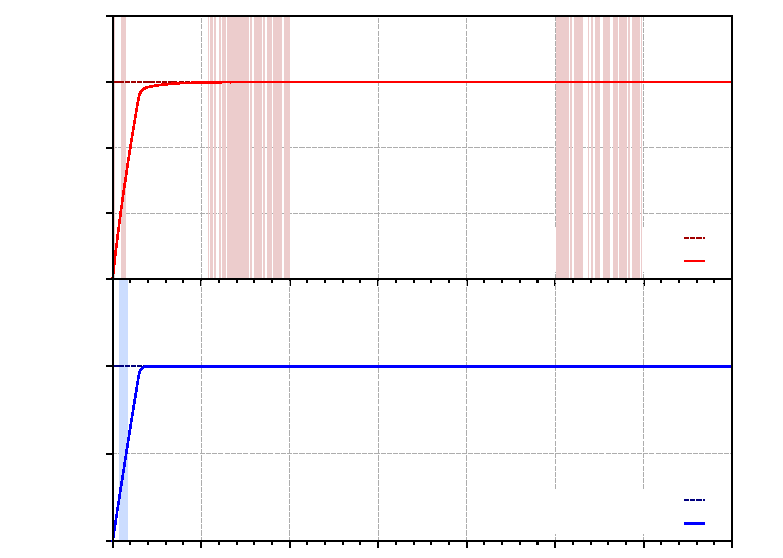
\includegraphics{fasr}}%
    \gplfronttext
  \end{picture}%
\endgroup
}
        \vspace{0.5cm}
        \caption{NSAF simulation -- Assumming a uniform distribution noise from
                 $\pm$2\%.}
        \label{fig:fasr}
    \end{minipage}
    \hfill
    \begin{minipage}[b]{0.48\linewidth}
        \scalebox{0.65}{% GNUPLOT: LaTeX picture with Postscript
\begingroup
  \makeatletter
  \providecommand\color[2][]{%
    \GenericError{(gnuplot) \space\space\space\@spaces}{%
      Package color not loaded in conjunction with
      terminal option `colourtext'%
    }{See the gnuplot documentation for explanation.%
    }{Either use 'blacktext' in gnuplot or load the package
      color.sty in LaTeX.}%
    \renewcommand\color[2][]{}%
  }%
  \providecommand\includegraphics[2][]{%
    \GenericError{(gnuplot) \space\space\space\@spaces}{%
      Package graphicx or graphics not loaded%
    }{See the gnuplot documentation for explanation.%
    }{The gnuplot epslatex terminal needs graphicx.sty or graphics.sty.}%
    \renewcommand\includegraphics[2][]{}%
  }%
  \providecommand\rotatebox[2]{#2}%
  \@ifundefined{ifGPcolor}{%
    \newif\ifGPcolor
    \GPcolortrue
  }{}%
  \@ifundefined{ifGPblacktext}{%
    \newif\ifGPblacktext
    \GPblacktexttrue
  }{}%
  % define a \g@addto@macro without @ in the name:
  \let\gplgaddtomacro\g@addto@macro
  % define empty templates for all commands taking text:
  \gdef\gplbacktext{}%
  \gdef\gplfronttext{}%
  \makeatother
  \ifGPblacktext
    % no textcolor at all
    \def\colorrgb#1{}%
    \def\colorgray#1{}%
  \else
    % gray or color?
    \ifGPcolor
      \def\colorrgb#1{\color[rgb]{#1}}%
      \def\colorgray#1{\color[gray]{#1}}%
      \expandafter\def\csname LTw\endcsname{\color{white}}%
      \expandafter\def\csname LTb\endcsname{\color{black}}%
      \expandafter\def\csname LTa\endcsname{\color{black}}%
      \expandafter\def\csname LT0\endcsname{\color[rgb]{1,0,0}}%
      \expandafter\def\csname LT1\endcsname{\color[rgb]{0,1,0}}%
      \expandafter\def\csname LT2\endcsname{\color[rgb]{0,0,1}}%
      \expandafter\def\csname LT3\endcsname{\color[rgb]{1,0,1}}%
      \expandafter\def\csname LT4\endcsname{\color[rgb]{0,1,1}}%
      \expandafter\def\csname LT5\endcsname{\color[rgb]{1,1,0}}%
      \expandafter\def\csname LT6\endcsname{\color[rgb]{0,0,0}}%
      \expandafter\def\csname LT7\endcsname{\color[rgb]{1,0.3,0}}%
      \expandafter\def\csname LT8\endcsname{\color[rgb]{0.5,0.5,0.5}}%
    \else
      % gray
      \def\colorrgb#1{\color{black}}%
      \def\colorgray#1{\color[gray]{#1}}%
      \expandafter\def\csname LTw\endcsname{\color{white}}%
      \expandafter\def\csname LTb\endcsname{\color{black}}%
      \expandafter\def\csname LTa\endcsname{\color{black}}%
      \expandafter\def\csname LT0\endcsname{\color{black}}%
      \expandafter\def\csname LT1\endcsname{\color{black}}%
      \expandafter\def\csname LT2\endcsname{\color{black}}%
      \expandafter\def\csname LT3\endcsname{\color{black}}%
      \expandafter\def\csname LT4\endcsname{\color{black}}%
      \expandafter\def\csname LT5\endcsname{\color{black}}%
      \expandafter\def\csname LT6\endcsname{\color{black}}%
      \expandafter\def\csname LT7\endcsname{\color{black}}%
      \expandafter\def\csname LT8\endcsname{\color{black}}%
    \fi
  \fi
  \setlength{\unitlength}{0.0500bp}%
  \begin{picture}(7200.00,5040.00)%
    \gplgaddtomacro\gplbacktext{%
      \csname LTb\endcsname%
      \put(726,2800){\makebox(0,0)[r]{\strut{} 5}}%
      \csname LTb\endcsname%
      \put(726,3080){\makebox(0,0)[r]{\strut{} 10}}%
      \csname LTb\endcsname%
      \put(726,3360){\makebox(0,0)[r]{\strut{} 15}}%
      \csname LTb\endcsname%
      \put(726,3640){\makebox(0,0)[r]{\strut{} 20}}%
      \csname LTb\endcsname%
      \put(726,3919){\makebox(0,0)[r]{\strut{} 25}}%
      \csname LTb\endcsname%
      \put(726,4199){\makebox(0,0)[r]{\strut{} 30}}%
      \csname LTb\endcsname%
      \put(726,4479){\makebox(0,0)[r]{\strut{} 35}}%
      \csname LTb\endcsname%
      \put(726,4759){\makebox(0,0)[r]{\strut{} 40}}%
      \csname LTb\endcsname%
      \put(726,5039){\makebox(0,0)[r]{\strut{} 45}}%
      \csname LTb\endcsname%
      \put(921,2237){\makebox(0,0){\strut{}}}%
      \csname LTb\endcsname%
      \put(1771,2237){\makebox(0,0){\strut{}}}%
      \csname LTb\endcsname%
      \put(2620,2237){\makebox(0,0){\strut{}}}%
      \csname LTb\endcsname%
      \put(3470,2237){\makebox(0,0){\strut{}}}%
      \csname LTb\endcsname%
      \put(4320,2237){\makebox(0,0){\strut{}}}%
      \csname LTb\endcsname%
      \put(5170,2237){\makebox(0,0){\strut{}}}%
      \csname LTb\endcsname%
      \put(6019,2237){\makebox(0,0){\strut{}}}%
      \csname LTb\endcsname%
      \put(6869,2237){\makebox(0,0){\strut{}}}%
      \put(352,3779){\rotatebox{-270}{\makebox(0,0){\strut{}Level [cm]}}}%
    }%
    \gplgaddtomacro\gplfronttext{%
      \csname LTb\endcsname%
      \put(6278,2913){\makebox(0,0)[r]{\strut{}Setpoint $T_1$}}%
      \csname LTb\endcsname%
      \put(6278,2693){\makebox(0,0)[r]{\strut{}Output $T_1$}}%
    }%
    \gplgaddtomacro\gplbacktext{%
      \csname LTb\endcsname%
      \put(726,0){\makebox(0,0)[r]{\strut{} 0}}%
      \csname LTb\endcsname%
      \put(726,315){\makebox(0,0)[r]{\strut{} 10}}%
      \csname LTb\endcsname%
      \put(726,630){\makebox(0,0)[r]{\strut{} 20}}%
      \csname LTb\endcsname%
      \put(726,945){\makebox(0,0)[r]{\strut{} 30}}%
      \csname LTb\endcsname%
      \put(726,1260){\makebox(0,0)[r]{\strut{} 40}}%
      \csname LTb\endcsname%
      \put(726,1575){\makebox(0,0)[r]{\strut{} 50}}%
      \csname LTb\endcsname%
      \put(726,1890){\makebox(0,0)[r]{\strut{} 60}}%
      \csname LTb\endcsname%
      \put(726,2205){\makebox(0,0)[r]{\strut{} 70}}%
      \csname LTb\endcsname%
      \put(726,2520){\makebox(0,0)[r]{\strut{} 80}}%
      \csname LTb\endcsname%
      \put(921,-283){\makebox(0,0){\strut{}0}}%
      \csname LTb\endcsname%
      \put(1771,-283){\makebox(0,0){\strut{}15}}%
      \csname LTb\endcsname%
      \put(2620,-283){\makebox(0,0){\strut{}30}}%
      \csname LTb\endcsname%
      \put(3470,-283){\makebox(0,0){\strut{}45}}%
      \csname LTb\endcsname%
      \put(4320,-283){\makebox(0,0){\strut{}60}}%
      \csname LTb\endcsname%
      \put(5170,-283){\makebox(0,0){\strut{}75}}%
      \csname LTb\endcsname%
      \put(6019,-283){\makebox(0,0){\strut{}90}}%
      \csname LTb\endcsname%
      \put(6869,-283){\makebox(0,0){\strut{}105}}%
      \put(352,1260){\rotatebox{-270}{\makebox(0,0){\strut{}Level [cm]}}}%
      \put(3895,-613){\makebox(0,0){\strut{}Time [s]}}%
    }%
    \gplgaddtomacro\gplfronttext{%
      \csname LTb\endcsname%
      \put(6278,393){\makebox(0,0)[r]{\strut{}Setpoint $T_2$}}%
      \csname LTb\endcsname%
      \put(6278,173){\makebox(0,0)[r]{\strut{}Output $T_2$}}%
    }%
    \gplbacktext
    \put(0,0){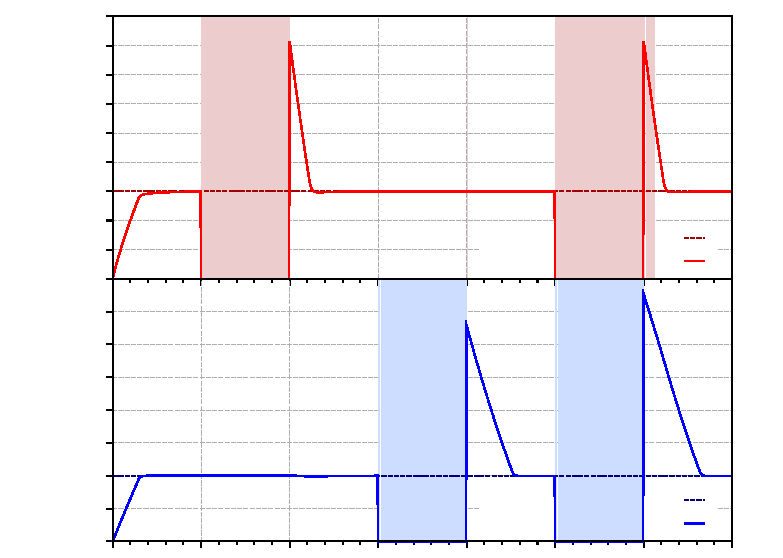
\includegraphics{fseq}}%
    \gplfronttext
  \end{picture}%
\endgroup
}
        \vspace{0.5cm}
        \caption{BSeF simulation -- Sensor's gain reduced to zero.}
        \label{fig:fseq}
    \end{minipage}
\end{figure}

Unlike the NSSeF, the simulation performed for the NSAF was not so easily
identified, as shown in Fig. \ref{fig:fasr}. The results obtained for $T_1$ can
even be considered reasonable, while the results for $T_2$ are clearly
unacceptable, given that none of the points at which the fault should have been
identified were recognized by the network. Nevertheless, the results are
consistent with the Tab. \ref{tab:best_ann}, where the total error exceeds 40\%.

As well as NNSeF, all other remaining faults were also easily identified by the
system, as shown in Figs. \ref{fig:fseq} to \ref{fig:fsivros}.

\begin{figure}[htb]
    \begin{minipage}[b]{0.48\linewidth}
        \scalebox{0.65}{% GNUPLOT: LaTeX picture with Postscript
\begingroup
  \makeatletter
  \providecommand\color[2][]{%
    \GenericError{(gnuplot) \space\space\space\@spaces}{%
      Package color not loaded in conjunction with
      terminal option `colourtext'%
    }{See the gnuplot documentation for explanation.%
    }{Either use 'blacktext' in gnuplot or load the package
      color.sty in LaTeX.}%
    \renewcommand\color[2][]{}%
  }%
  \providecommand\includegraphics[2][]{%
    \GenericError{(gnuplot) \space\space\space\@spaces}{%
      Package graphicx or graphics not loaded%
    }{See the gnuplot documentation for explanation.%
    }{The gnuplot epslatex terminal needs graphicx.sty or graphics.sty.}%
    \renewcommand\includegraphics[2][]{}%
  }%
  \providecommand\rotatebox[2]{#2}%
  \@ifundefined{ifGPcolor}{%
    \newif\ifGPcolor
    \GPcolortrue
  }{}%
  \@ifundefined{ifGPblacktext}{%
    \newif\ifGPblacktext
    \GPblacktexttrue
  }{}%
  % define a \g@addto@macro without @ in the name:
  \let\gplgaddtomacro\g@addto@macro
  % define empty templates for all commands taking text:
  \gdef\gplbacktext{}%
  \gdef\gplfronttext{}%
  \makeatother
  \ifGPblacktext
    % no textcolor at all
    \def\colorrgb#1{}%
    \def\colorgray#1{}%
  \else
    % gray or color?
    \ifGPcolor
      \def\colorrgb#1{\color[rgb]{#1}}%
      \def\colorgray#1{\color[gray]{#1}}%
      \expandafter\def\csname LTw\endcsname{\color{white}}%
      \expandafter\def\csname LTb\endcsname{\color{black}}%
      \expandafter\def\csname LTa\endcsname{\color{black}}%
      \expandafter\def\csname LT0\endcsname{\color[rgb]{1,0,0}}%
      \expandafter\def\csname LT1\endcsname{\color[rgb]{0,1,0}}%
      \expandafter\def\csname LT2\endcsname{\color[rgb]{0,0,1}}%
      \expandafter\def\csname LT3\endcsname{\color[rgb]{1,0,1}}%
      \expandafter\def\csname LT4\endcsname{\color[rgb]{0,1,1}}%
      \expandafter\def\csname LT5\endcsname{\color[rgb]{1,1,0}}%
      \expandafter\def\csname LT6\endcsname{\color[rgb]{0,0,0}}%
      \expandafter\def\csname LT7\endcsname{\color[rgb]{1,0.3,0}}%
      \expandafter\def\csname LT8\endcsname{\color[rgb]{0.5,0.5,0.5}}%
    \else
      % gray
      \def\colorrgb#1{\color{black}}%
      \def\colorgray#1{\color[gray]{#1}}%
      \expandafter\def\csname LTw\endcsname{\color{white}}%
      \expandafter\def\csname LTb\endcsname{\color{black}}%
      \expandafter\def\csname LTa\endcsname{\color{black}}%
      \expandafter\def\csname LT0\endcsname{\color{black}}%
      \expandafter\def\csname LT1\endcsname{\color{black}}%
      \expandafter\def\csname LT2\endcsname{\color{black}}%
      \expandafter\def\csname LT3\endcsname{\color{black}}%
      \expandafter\def\csname LT4\endcsname{\color{black}}%
      \expandafter\def\csname LT5\endcsname{\color{black}}%
      \expandafter\def\csname LT6\endcsname{\color{black}}%
      \expandafter\def\csname LT7\endcsname{\color{black}}%
      \expandafter\def\csname LT8\endcsname{\color{black}}%
    \fi
  \fi
  \setlength{\unitlength}{0.0500bp}%
  \begin{picture}(7200.00,5040.00)%
    \gplgaddtomacro\gplbacktext{%
      \csname LTb\endcsname%
      \put(726,3150){\makebox(0,0)[r]{\strut{} 5}}%
      \csname LTb\endcsname%
      \put(726,3780){\makebox(0,0)[r]{\strut{} 10}}%
      \csname LTb\endcsname%
      \put(726,4409){\makebox(0,0)[r]{\strut{} 15}}%
      \csname LTb\endcsname%
      \put(726,5039){\makebox(0,0)[r]{\strut{} 20}}%
      \csname LTb\endcsname%
      \put(921,2237){\makebox(0,0){\strut{}}}%
      \csname LTb\endcsname%
      \put(1771,2237){\makebox(0,0){\strut{}}}%
      \csname LTb\endcsname%
      \put(2620,2237){\makebox(0,0){\strut{}}}%
      \csname LTb\endcsname%
      \put(3470,2237){\makebox(0,0){\strut{}}}%
      \csname LTb\endcsname%
      \put(4320,2237){\makebox(0,0){\strut{}}}%
      \csname LTb\endcsname%
      \put(5170,2237){\makebox(0,0){\strut{}}}%
      \csname LTb\endcsname%
      \put(6019,2237){\makebox(0,0){\strut{}}}%
      \csname LTb\endcsname%
      \put(6869,2237){\makebox(0,0){\strut{}}}%
      \put(352,3779){\rotatebox{-270}{\makebox(0,0){\strut{}Nível [cm]}}}%
    }%
    \gplgaddtomacro\gplfronttext{%
      \csname LTb\endcsname%
      \put(6278,2913){\makebox(0,0)[r]{\strut{}Ref. $T_1$}}%
      \csname LTb\endcsname%
      \put(6278,2693){\makebox(0,0)[r]{\strut{}Saída $T_1$}}%
    }%
    \gplgaddtomacro\gplbacktext{%
      \csname LTb\endcsname%
      \put(726,0){\makebox(0,0)[r]{\strut{} 0}}%
      \csname LTb\endcsname%
      \put(726,840){\makebox(0,0)[r]{\strut{} 10}}%
      \csname LTb\endcsname%
      \put(726,1680){\makebox(0,0)[r]{\strut{} 20}}%
      \csname LTb\endcsname%
      \put(726,2520){\makebox(0,0)[r]{\strut{} 30}}%
      \csname LTb\endcsname%
      \put(921,-283){\makebox(0,0){\strut{}0}}%
      \csname LTb\endcsname%
      \put(1771,-283){\makebox(0,0){\strut{}15}}%
      \csname LTb\endcsname%
      \put(2620,-283){\makebox(0,0){\strut{}30}}%
      \csname LTb\endcsname%
      \put(3470,-283){\makebox(0,0){\strut{}45}}%
      \csname LTb\endcsname%
      \put(4320,-283){\makebox(0,0){\strut{}60}}%
      \csname LTb\endcsname%
      \put(5170,-283){\makebox(0,0){\strut{}75}}%
      \csname LTb\endcsname%
      \put(6019,-283){\makebox(0,0){\strut{}90}}%
      \csname LTb\endcsname%
      \put(6869,-283){\makebox(0,0){\strut{}105}}%
      \put(352,1260){\rotatebox{-270}{\makebox(0,0){\strut{}Nível [cm]}}}%
      \put(3895,-613){\makebox(0,0){\strut{}Tempo [s]}}%
    }%
    \gplgaddtomacro\gplfronttext{%
      \csname LTb\endcsname%
      \put(6278,393){\makebox(0,0)[r]{\strut{}Ref. $T_2$}}%
      \csname LTb\endcsname%
      \put(6278,173){\makebox(0,0)[r]{\strut{}Saída $T_2$}}%
    }%
    \gplbacktext
    \put(0,0){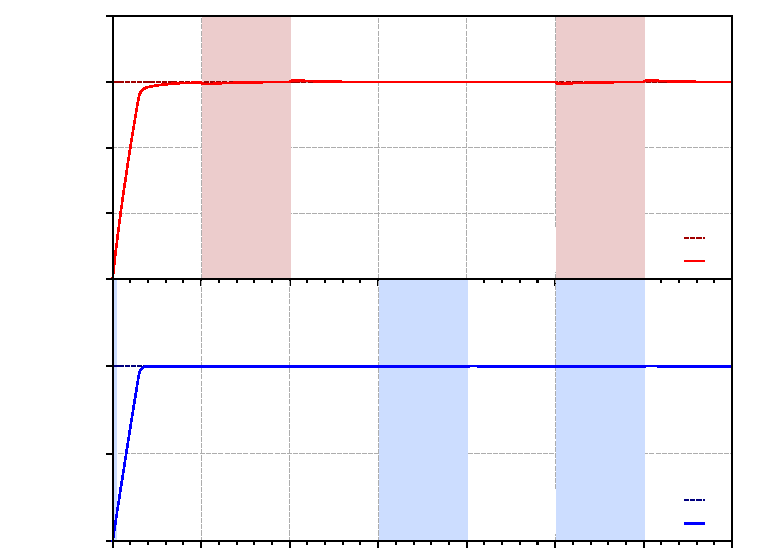
\includegraphics{fadg}}%
    \gplfronttext
  \end{picture}%
\endgroup
}
        \vspace{0.5cm}
        \caption{UGAF simulation -- Actuator's gain reduced to 80\% from the
                 default value.}
        \label{fig:fadg}
    \end{minipage}
    \hfill
    \begin{minipage}[b]{0.48\linewidth}
        \scalebox{0.65}{% GNUPLOT: LaTeX picture with Postscript
\begingroup
  \makeatletter
  \providecommand\color[2][]{%
    \GenericError{(gnuplot) \space\space\space\@spaces}{%
      Package color not loaded in conjunction with
      terminal option `colourtext'%
    }{See the gnuplot documentation for explanation.%
    }{Either use 'blacktext' in gnuplot or load the package
      color.sty in LaTeX.}%
    \renewcommand\color[2][]{}%
  }%
  \providecommand\includegraphics[2][]{%
    \GenericError{(gnuplot) \space\space\space\@spaces}{%
      Package graphicx or graphics not loaded%
    }{See the gnuplot documentation for explanation.%
    }{The gnuplot epslatex terminal needs graphicx.sty or graphics.sty.}%
    \renewcommand\includegraphics[2][]{}%
  }%
  \providecommand\rotatebox[2]{#2}%
  \@ifundefined{ifGPcolor}{%
    \newif\ifGPcolor
    \GPcolortrue
  }{}%
  \@ifundefined{ifGPblacktext}{%
    \newif\ifGPblacktext
    \GPblacktexttrue
  }{}%
  % define a \g@addto@macro without @ in the name:
  \let\gplgaddtomacro\g@addto@macro
  % define empty templates for all commands taking text:
  \gdef\gplbacktext{}%
  \gdef\gplfronttext{}%
  \makeatother
  \ifGPblacktext
    % no textcolor at all
    \def\colorrgb#1{}%
    \def\colorgray#1{}%
  \else
    % gray or color?
    \ifGPcolor
      \def\colorrgb#1{\color[rgb]{#1}}%
      \def\colorgray#1{\color[gray]{#1}}%
      \expandafter\def\csname LTw\endcsname{\color{white}}%
      \expandafter\def\csname LTb\endcsname{\color{black}}%
      \expandafter\def\csname LTa\endcsname{\color{black}}%
      \expandafter\def\csname LT0\endcsname{\color[rgb]{1,0,0}}%
      \expandafter\def\csname LT1\endcsname{\color[rgb]{0,1,0}}%
      \expandafter\def\csname LT2\endcsname{\color[rgb]{0,0,1}}%
      \expandafter\def\csname LT3\endcsname{\color[rgb]{1,0,1}}%
      \expandafter\def\csname LT4\endcsname{\color[rgb]{0,1,1}}%
      \expandafter\def\csname LT5\endcsname{\color[rgb]{1,1,0}}%
      \expandafter\def\csname LT6\endcsname{\color[rgb]{0,0,0}}%
      \expandafter\def\csname LT7\endcsname{\color[rgb]{1,0.3,0}}%
      \expandafter\def\csname LT8\endcsname{\color[rgb]{0.5,0.5,0.5}}%
    \else
      % gray
      \def\colorrgb#1{\color{black}}%
      \def\colorgray#1{\color[gray]{#1}}%
      \expandafter\def\csname LTw\endcsname{\color{white}}%
      \expandafter\def\csname LTb\endcsname{\color{black}}%
      \expandafter\def\csname LTa\endcsname{\color{black}}%
      \expandafter\def\csname LT0\endcsname{\color{black}}%
      \expandafter\def\csname LT1\endcsname{\color{black}}%
      \expandafter\def\csname LT2\endcsname{\color{black}}%
      \expandafter\def\csname LT3\endcsname{\color{black}}%
      \expandafter\def\csname LT4\endcsname{\color{black}}%
      \expandafter\def\csname LT5\endcsname{\color{black}}%
      \expandafter\def\csname LT6\endcsname{\color{black}}%
      \expandafter\def\csname LT7\endcsname{\color{black}}%
      \expandafter\def\csname LT8\endcsname{\color{black}}%
    \fi
  \fi
  \setlength{\unitlength}{0.0500bp}%
  \begin{picture}(7200.00,5040.00)%
    \gplgaddtomacro\gplbacktext{%
      \csname LTb\endcsname%
      \put(726,3150){\makebox(0,0)[r]{\strut{} 5}}%
      \csname LTb\endcsname%
      \put(726,3780){\makebox(0,0)[r]{\strut{} 10}}%
      \csname LTb\endcsname%
      \put(726,4409){\makebox(0,0)[r]{\strut{} 15}}%
      \csname LTb\endcsname%
      \put(726,5039){\makebox(0,0)[r]{\strut{} 20}}%
      \csname LTb\endcsname%
      \put(921,2237){\makebox(0,0){\strut{}}}%
      \csname LTb\endcsname%
      \put(1771,2237){\makebox(0,0){\strut{}}}%
      \csname LTb\endcsname%
      \put(2620,2237){\makebox(0,0){\strut{}}}%
      \csname LTb\endcsname%
      \put(3470,2237){\makebox(0,0){\strut{}}}%
      \csname LTb\endcsname%
      \put(4320,2237){\makebox(0,0){\strut{}}}%
      \csname LTb\endcsname%
      \put(5170,2237){\makebox(0,0){\strut{}}}%
      \csname LTb\endcsname%
      \put(6019,2237){\makebox(0,0){\strut{}}}%
      \csname LTb\endcsname%
      \put(6869,2237){\makebox(0,0){\strut{}}}%
      \put(352,3779){\rotatebox{-270}{\makebox(0,0){\strut{}Level [cm]}}}%
    }%
    \gplgaddtomacro\gplfronttext{%
      \csname LTb\endcsname%
      \put(6278,2913){\makebox(0,0)[r]{\strut{}Setpoint $T_1$}}%
      \csname LTb\endcsname%
      \put(6278,2693){\makebox(0,0)[r]{\strut{}Output $T_1$}}%
    }%
    \gplgaddtomacro\gplbacktext{%
      \csname LTb\endcsname%
      \put(726,0){\makebox(0,0)[r]{\strut{} 0}}%
      \csname LTb\endcsname%
      \put(726,840){\makebox(0,0)[r]{\strut{} 10}}%
      \csname LTb\endcsname%
      \put(726,1680){\makebox(0,0)[r]{\strut{} 20}}%
      \csname LTb\endcsname%
      \put(726,2520){\makebox(0,0)[r]{\strut{} 30}}%
      \csname LTb\endcsname%
      \put(921,-283){\makebox(0,0){\strut{}0}}%
      \csname LTb\endcsname%
      \put(1771,-283){\makebox(0,0){\strut{}15}}%
      \csname LTb\endcsname%
      \put(2620,-283){\makebox(0,0){\strut{}30}}%
      \csname LTb\endcsname%
      \put(3470,-283){\makebox(0,0){\strut{}45}}%
      \csname LTb\endcsname%
      \put(4320,-283){\makebox(0,0){\strut{}60}}%
      \csname LTb\endcsname%
      \put(5170,-283){\makebox(0,0){\strut{}75}}%
      \csname LTb\endcsname%
      \put(6019,-283){\makebox(0,0){\strut{}90}}%
      \csname LTb\endcsname%
      \put(6869,-283){\makebox(0,0){\strut{}105}}%
      \put(352,1260){\rotatebox{-270}{\makebox(0,0){\strut{}Level [cm]}}}%
      \put(3895,-613){\makebox(0,0){\strut{}Time [s]}}%
    }%
    \gplgaddtomacro\gplfronttext{%
      \csname LTb\endcsname%
      \put(6278,393){\makebox(0,0)[r]{\strut{}Setpoint $T_2$}}%
      \csname LTb\endcsname%
      \put(6278,173){\makebox(0,0)[r]{\strut{}Output $T_2$}}%
    }%
    \gplbacktext
    \put(0,0){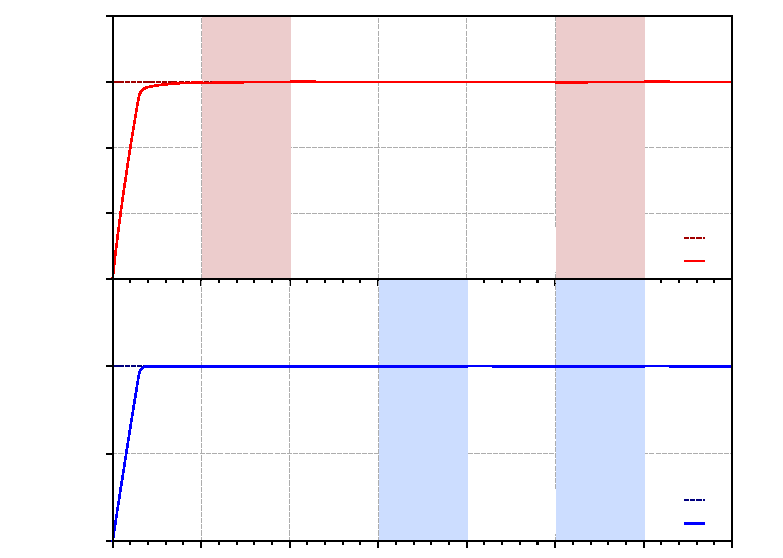
\includegraphics{fado}}%
    \gplfronttext
  \end{picture}%
\endgroup
}
        \vspace{0.5cm}
        \caption{UOAF simulation -- Actuator's offset configured to $-0.5$
                 Volts.}
        \label{fig:fado}
    \end{minipage}
\end{figure}

\begin{figure}[htb]
    \begin{minipage}[b]{0.48\linewidth}
        \scalebox{0.65}{% GNUPLOT: LaTeX picture with Postscript
\begingroup
  \makeatletter
  \providecommand\color[2][]{%
    \GenericError{(gnuplot) \space\space\space\@spaces}{%
      Package color not loaded in conjunction with
      terminal option `colourtext'%
    }{See the gnuplot documentation for explanation.%
    }{Either use 'blacktext' in gnuplot or load the package
      color.sty in LaTeX.}%
    \renewcommand\color[2][]{}%
  }%
  \providecommand\includegraphics[2][]{%
    \GenericError{(gnuplot) \space\space\space\@spaces}{%
      Package graphicx or graphics not loaded%
    }{See the gnuplot documentation for explanation.%
    }{The gnuplot epslatex terminal needs graphicx.sty or graphics.sty.}%
    \renewcommand\includegraphics[2][]{}%
  }%
  \providecommand\rotatebox[2]{#2}%
  \@ifundefined{ifGPcolor}{%
    \newif\ifGPcolor
    \GPcolortrue
  }{}%
  \@ifundefined{ifGPblacktext}{%
    \newif\ifGPblacktext
    \GPblacktexttrue
  }{}%
  % define a \g@addto@macro without @ in the name:
  \let\gplgaddtomacro\g@addto@macro
  % define empty templates for all commands taking text:
  \gdef\gplbacktext{}%
  \gdef\gplfronttext{}%
  \makeatother
  \ifGPblacktext
    % no textcolor at all
    \def\colorrgb#1{}%
    \def\colorgray#1{}%
  \else
    % gray or color?
    \ifGPcolor
      \def\colorrgb#1{\color[rgb]{#1}}%
      \def\colorgray#1{\color[gray]{#1}}%
      \expandafter\def\csname LTw\endcsname{\color{white}}%
      \expandafter\def\csname LTb\endcsname{\color{black}}%
      \expandafter\def\csname LTa\endcsname{\color{black}}%
      \expandafter\def\csname LT0\endcsname{\color[rgb]{1,0,0}}%
      \expandafter\def\csname LT1\endcsname{\color[rgb]{0,1,0}}%
      \expandafter\def\csname LT2\endcsname{\color[rgb]{0,0,1}}%
      \expandafter\def\csname LT3\endcsname{\color[rgb]{1,0,1}}%
      \expandafter\def\csname LT4\endcsname{\color[rgb]{0,1,1}}%
      \expandafter\def\csname LT5\endcsname{\color[rgb]{1,1,0}}%
      \expandafter\def\csname LT6\endcsname{\color[rgb]{0,0,0}}%
      \expandafter\def\csname LT7\endcsname{\color[rgb]{1,0.3,0}}%
      \expandafter\def\csname LT8\endcsname{\color[rgb]{0.5,0.5,0.5}}%
    \else
      % gray
      \def\colorrgb#1{\color{black}}%
      \def\colorgray#1{\color[gray]{#1}}%
      \expandafter\def\csname LTw\endcsname{\color{white}}%
      \expandafter\def\csname LTb\endcsname{\color{black}}%
      \expandafter\def\csname LTa\endcsname{\color{black}}%
      \expandafter\def\csname LT0\endcsname{\color{black}}%
      \expandafter\def\csname LT1\endcsname{\color{black}}%
      \expandafter\def\csname LT2\endcsname{\color{black}}%
      \expandafter\def\csname LT3\endcsname{\color{black}}%
      \expandafter\def\csname LT4\endcsname{\color{black}}%
      \expandafter\def\csname LT5\endcsname{\color{black}}%
      \expandafter\def\csname LT6\endcsname{\color{black}}%
      \expandafter\def\csname LT7\endcsname{\color{black}}%
      \expandafter\def\csname LT8\endcsname{\color{black}}%
    \fi
  \fi
  \setlength{\unitlength}{0.0500bp}%
  \begin{picture}(7200.00,5040.00)%
    \gplgaddtomacro\gplbacktext{%
      \csname LTb\endcsname%
      \put(726,3150){\makebox(0,0)[r]{\strut{} 5}}%
      \csname LTb\endcsname%
      \put(726,3780){\makebox(0,0)[r]{\strut{} 10}}%
      \csname LTb\endcsname%
      \put(726,4409){\makebox(0,0)[r]{\strut{} 15}}%
      \csname LTb\endcsname%
      \put(726,5039){\makebox(0,0)[r]{\strut{} 20}}%
      \csname LTb\endcsname%
      \put(921,2237){\makebox(0,0){\strut{}}}%
      \csname LTb\endcsname%
      \put(1771,2237){\makebox(0,0){\strut{}}}%
      \csname LTb\endcsname%
      \put(2620,2237){\makebox(0,0){\strut{}}}%
      \csname LTb\endcsname%
      \put(3470,2237){\makebox(0,0){\strut{}}}%
      \csname LTb\endcsname%
      \put(4320,2237){\makebox(0,0){\strut{}}}%
      \csname LTb\endcsname%
      \put(5170,2237){\makebox(0,0){\strut{}}}%
      \csname LTb\endcsname%
      \put(6019,2237){\makebox(0,0){\strut{}}}%
      \csname LTb\endcsname%
      \put(6869,2237){\makebox(0,0){\strut{}}}%
      \put(352,3779){\rotatebox{-270}{\makebox(0,0){\strut{}Nível [cm]}}}%
    }%
    \gplgaddtomacro\gplfronttext{%
      \csname LTb\endcsname%
      \put(6278,2913){\makebox(0,0)[r]{\strut{}Ref. $T_1$}}%
      \csname LTb\endcsname%
      \put(6278,2693){\makebox(0,0)[r]{\strut{}Saída $T_1$}}%
    }%
    \gplgaddtomacro\gplbacktext{%
      \csname LTb\endcsname%
      \put(726,0){\makebox(0,0)[r]{\strut{} 0}}%
      \csname LTb\endcsname%
      \put(726,840){\makebox(0,0)[r]{\strut{} 10}}%
      \csname LTb\endcsname%
      \put(726,1680){\makebox(0,0)[r]{\strut{} 20}}%
      \csname LTb\endcsname%
      \put(726,2520){\makebox(0,0)[r]{\strut{} 30}}%
      \csname LTb\endcsname%
      \put(921,-283){\makebox(0,0){\strut{}0}}%
      \csname LTb\endcsname%
      \put(1771,-283){\makebox(0,0){\strut{}15}}%
      \csname LTb\endcsname%
      \put(2620,-283){\makebox(0,0){\strut{}30}}%
      \csname LTb\endcsname%
      \put(3470,-283){\makebox(0,0){\strut{}45}}%
      \csname LTb\endcsname%
      \put(4320,-283){\makebox(0,0){\strut{}60}}%
      \csname LTb\endcsname%
      \put(5170,-283){\makebox(0,0){\strut{}75}}%
      \csname LTb\endcsname%
      \put(6019,-283){\makebox(0,0){\strut{}90}}%
      \csname LTb\endcsname%
      \put(6869,-283){\makebox(0,0){\strut{}105}}%
      \put(352,1260){\rotatebox{-270}{\makebox(0,0){\strut{}Nível [cm]}}}%
      \put(3895,-613){\makebox(0,0){\strut{}Tempo [s]}}%
    }%
    \gplgaddtomacro\gplfronttext{%
      \csname LTb\endcsname%
      \put(6278,393){\makebox(0,0)[r]{\strut{}Ref. $T_2$}}%
      \csname LTb\endcsname%
      \put(6278,173){\makebox(0,0)[r]{\strut{}Saída $T_2$}}%
    }%
    \gplbacktext
    \put(0,0){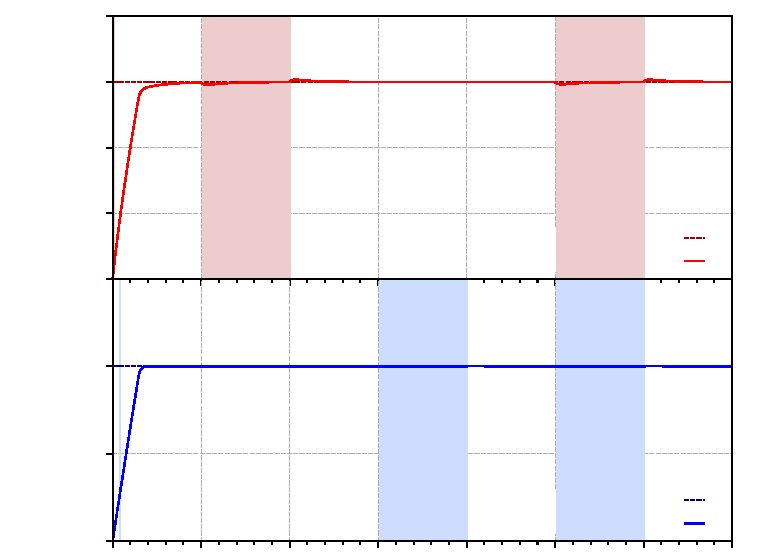
\includegraphics{favk}}%
    \gplfronttext
  \end{picture}%
\endgroup
}
        \vspace{0.5cm}
        \caption{$K_m$AF simulation -- $K_m$ reduced to 75\% from the default
                 value.}
        \label{fig:favk}
    \end{minipage}
    \hfill
    \begin{minipage}[b]{0.48\linewidth}
        \scalebox{0.65}{% GNUPLOT: LaTeX picture with Postscript
\begingroup
  \makeatletter
  \providecommand\color[2][]{%
    \GenericError{(gnuplot) \space\space\space\@spaces}{%
      Package color not loaded in conjunction with
      terminal option `colourtext'%
    }{See the gnuplot documentation for explanation.%
    }{Either use 'blacktext' in gnuplot or load the package
      color.sty in LaTeX.}%
    \renewcommand\color[2][]{}%
  }%
  \providecommand\includegraphics[2][]{%
    \GenericError{(gnuplot) \space\space\space\@spaces}{%
      Package graphicx or graphics not loaded%
    }{See the gnuplot documentation for explanation.%
    }{The gnuplot epslatex terminal needs graphicx.sty or graphics.sty.}%
    \renewcommand\includegraphics[2][]{}%
  }%
  \providecommand\rotatebox[2]{#2}%
  \@ifundefined{ifGPcolor}{%
    \newif\ifGPcolor
    \GPcolortrue
  }{}%
  \@ifundefined{ifGPblacktext}{%
    \newif\ifGPblacktext
    \GPblacktexttrue
  }{}%
  % define a \g@addto@macro without @ in the name:
  \let\gplgaddtomacro\g@addto@macro
  % define empty templates for all commands taking text:
  \gdef\gplbacktext{}%
  \gdef\gplfronttext{}%
  \makeatother
  \ifGPblacktext
    % no textcolor at all
    \def\colorrgb#1{}%
    \def\colorgray#1{}%
  \else
    % gray or color?
    \ifGPcolor
      \def\colorrgb#1{\color[rgb]{#1}}%
      \def\colorgray#1{\color[gray]{#1}}%
      \expandafter\def\csname LTw\endcsname{\color{white}}%
      \expandafter\def\csname LTb\endcsname{\color{black}}%
      \expandafter\def\csname LTa\endcsname{\color{black}}%
      \expandafter\def\csname LT0\endcsname{\color[rgb]{1,0,0}}%
      \expandafter\def\csname LT1\endcsname{\color[rgb]{0,1,0}}%
      \expandafter\def\csname LT2\endcsname{\color[rgb]{0,0,1}}%
      \expandafter\def\csname LT3\endcsname{\color[rgb]{1,0,1}}%
      \expandafter\def\csname LT4\endcsname{\color[rgb]{0,1,1}}%
      \expandafter\def\csname LT5\endcsname{\color[rgb]{1,1,0}}%
      \expandafter\def\csname LT6\endcsname{\color[rgb]{0,0,0}}%
      \expandafter\def\csname LT7\endcsname{\color[rgb]{1,0.3,0}}%
      \expandafter\def\csname LT8\endcsname{\color[rgb]{0.5,0.5,0.5}}%
    \else
      % gray
      \def\colorrgb#1{\color{black}}%
      \def\colorgray#1{\color[gray]{#1}}%
      \expandafter\def\csname LTw\endcsname{\color{white}}%
      \expandafter\def\csname LTb\endcsname{\color{black}}%
      \expandafter\def\csname LTa\endcsname{\color{black}}%
      \expandafter\def\csname LT0\endcsname{\color{black}}%
      \expandafter\def\csname LT1\endcsname{\color{black}}%
      \expandafter\def\csname LT2\endcsname{\color{black}}%
      \expandafter\def\csname LT3\endcsname{\color{black}}%
      \expandafter\def\csname LT4\endcsname{\color{black}}%
      \expandafter\def\csname LT5\endcsname{\color{black}}%
      \expandafter\def\csname LT6\endcsname{\color{black}}%
      \expandafter\def\csname LT7\endcsname{\color{black}}%
      \expandafter\def\csname LT8\endcsname{\color{black}}%
    \fi
  \fi
  \setlength{\unitlength}{0.0500bp}%
  \begin{picture}(7200.00,5040.00)%
    \gplgaddtomacro\gplbacktext{%
      \csname LTb\endcsname%
      \put(726,3150){\makebox(0,0)[r]{\strut{} 5}}%
      \csname LTb\endcsname%
      \put(726,3780){\makebox(0,0)[r]{\strut{} 10}}%
      \csname LTb\endcsname%
      \put(726,4409){\makebox(0,0)[r]{\strut{} 15}}%
      \csname LTb\endcsname%
      \put(726,5039){\makebox(0,0)[r]{\strut{} 20}}%
      \csname LTb\endcsname%
      \put(921,2237){\makebox(0,0){\strut{}}}%
      \csname LTb\endcsname%
      \put(1771,2237){\makebox(0,0){\strut{}}}%
      \csname LTb\endcsname%
      \put(2620,2237){\makebox(0,0){\strut{}}}%
      \csname LTb\endcsname%
      \put(3470,2237){\makebox(0,0){\strut{}}}%
      \csname LTb\endcsname%
      \put(4320,2237){\makebox(0,0){\strut{}}}%
      \csname LTb\endcsname%
      \put(5170,2237){\makebox(0,0){\strut{}}}%
      \csname LTb\endcsname%
      \put(6019,2237){\makebox(0,0){\strut{}}}%
      \csname LTb\endcsname%
      \put(6869,2237){\makebox(0,0){\strut{}}}%
      \put(352,3779){\rotatebox{-270}{\makebox(0,0){\strut{}Level [cm]}}}%
    }%
    \gplgaddtomacro\gplfronttext{%
      \csname LTb\endcsname%
      \put(6278,2913){\makebox(0,0)[r]{\strut{}Setpoint $T_1$}}%
      \csname LTb\endcsname%
      \put(6278,2693){\makebox(0,0)[r]{\strut{}Output $T_1$}}%
    }%
    \gplgaddtomacro\gplbacktext{%
      \csname LTb\endcsname%
      \put(726,0){\makebox(0,0)[r]{\strut{} 0}}%
      \csname LTb\endcsname%
      \put(726,840){\makebox(0,0)[r]{\strut{} 10}}%
      \csname LTb\endcsname%
      \put(726,1680){\makebox(0,0)[r]{\strut{} 20}}%
      \csname LTb\endcsname%
      \put(726,2520){\makebox(0,0)[r]{\strut{} 30}}%
      \csname LTb\endcsname%
      \put(921,-283){\makebox(0,0){\strut{}0}}%
      \csname LTb\endcsname%
      \put(1771,-283){\makebox(0,0){\strut{}15}}%
      \csname LTb\endcsname%
      \put(2620,-283){\makebox(0,0){\strut{}30}}%
      \csname LTb\endcsname%
      \put(3470,-283){\makebox(0,0){\strut{}45}}%
      \csname LTb\endcsname%
      \put(4320,-283){\makebox(0,0){\strut{}60}}%
      \csname LTb\endcsname%
      \put(5170,-283){\makebox(0,0){\strut{}75}}%
      \csname LTb\endcsname%
      \put(6019,-283){\makebox(0,0){\strut{}90}}%
      \csname LTb\endcsname%
      \put(6869,-283){\makebox(0,0){\strut{}105}}%
      \put(352,1260){\rotatebox{-270}{\makebox(0,0){\strut{}Level [cm]}}}%
      \put(3895,-613){\makebox(0,0){\strut{}Time [s]}}%
    }%
    \gplgaddtomacro\gplfronttext{%
      \csname LTb\endcsname%
      \put(6278,393){\makebox(0,0)[r]{\strut{}Setpoint $T_2$}}%
      \csname LTb\endcsname%
      \put(6278,173){\makebox(0,0)[r]{\strut{}Output $T_2$}}%
    }%
    \gplbacktext
    \put(0,0){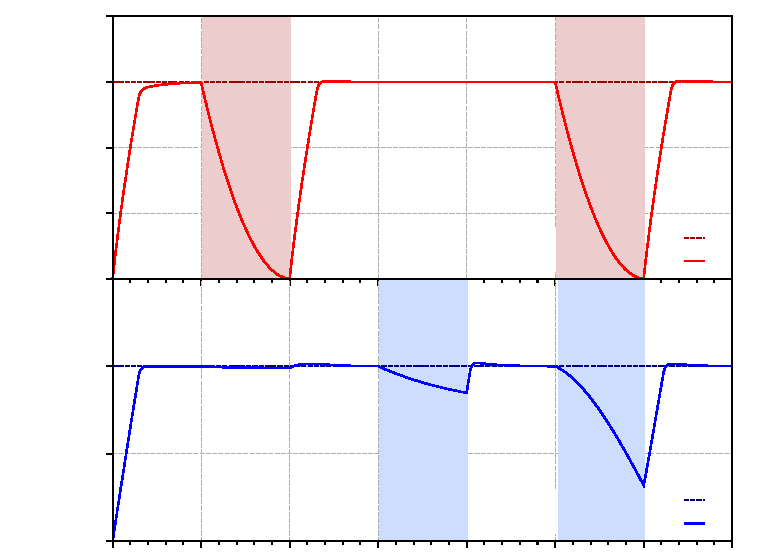
\includegraphics{faq}}%
    \gplfronttext
  \end{picture}%
\endgroup
}
        \vspace{0.5cm}
        \caption{BAF simulation -- Actuator's gain reduced to zero.}
        \label{fig:faq}
    \end{minipage}
\end{figure}

\begin{figure}[htb]
    \begin{minipage}[b]{0.48\linewidth}
        \scalebox{0.65}{% GNUPLOT: LaTeX picture with Postscript
\begingroup
  \makeatletter
  \providecommand\color[2][]{%
    \GenericError{(gnuplot) \space\space\space\@spaces}{%
      Package color not loaded in conjunction with
      terminal option `colourtext'%
    }{See the gnuplot documentation for explanation.%
    }{Either use 'blacktext' in gnuplot or load the package
      color.sty in LaTeX.}%
    \renewcommand\color[2][]{}%
  }%
  \providecommand\includegraphics[2][]{%
    \GenericError{(gnuplot) \space\space\space\@spaces}{%
      Package graphicx or graphics not loaded%
    }{See the gnuplot documentation for explanation.%
    }{The gnuplot epslatex terminal needs graphicx.sty or graphics.sty.}%
    \renewcommand\includegraphics[2][]{}%
  }%
  \providecommand\rotatebox[2]{#2}%
  \@ifundefined{ifGPcolor}{%
    \newif\ifGPcolor
    \GPcolortrue
  }{}%
  \@ifundefined{ifGPblacktext}{%
    \newif\ifGPblacktext
    \GPblacktexttrue
  }{}%
  % define a \g@addto@macro without @ in the name:
  \let\gplgaddtomacro\g@addto@macro
  % define empty templates for all commands taking text:
  \gdef\gplbacktext{}%
  \gdef\gplfronttext{}%
  \makeatother
  \ifGPblacktext
    % no textcolor at all
    \def\colorrgb#1{}%
    \def\colorgray#1{}%
  \else
    % gray or color?
    \ifGPcolor
      \def\colorrgb#1{\color[rgb]{#1}}%
      \def\colorgray#1{\color[gray]{#1}}%
      \expandafter\def\csname LTw\endcsname{\color{white}}%
      \expandafter\def\csname LTb\endcsname{\color{black}}%
      \expandafter\def\csname LTa\endcsname{\color{black}}%
      \expandafter\def\csname LT0\endcsname{\color[rgb]{1,0,0}}%
      \expandafter\def\csname LT1\endcsname{\color[rgb]{0,1,0}}%
      \expandafter\def\csname LT2\endcsname{\color[rgb]{0,0,1}}%
      \expandafter\def\csname LT3\endcsname{\color[rgb]{1,0,1}}%
      \expandafter\def\csname LT4\endcsname{\color[rgb]{0,1,1}}%
      \expandafter\def\csname LT5\endcsname{\color[rgb]{1,1,0}}%
      \expandafter\def\csname LT6\endcsname{\color[rgb]{0,0,0}}%
      \expandafter\def\csname LT7\endcsname{\color[rgb]{1,0.3,0}}%
      \expandafter\def\csname LT8\endcsname{\color[rgb]{0.5,0.5,0.5}}%
    \else
      % gray
      \def\colorrgb#1{\color{black}}%
      \def\colorgray#1{\color[gray]{#1}}%
      \expandafter\def\csname LTw\endcsname{\color{white}}%
      \expandafter\def\csname LTb\endcsname{\color{black}}%
      \expandafter\def\csname LTa\endcsname{\color{black}}%
      \expandafter\def\csname LT0\endcsname{\color{black}}%
      \expandafter\def\csname LT1\endcsname{\color{black}}%
      \expandafter\def\csname LT2\endcsname{\color{black}}%
      \expandafter\def\csname LT3\endcsname{\color{black}}%
      \expandafter\def\csname LT4\endcsname{\color{black}}%
      \expandafter\def\csname LT5\endcsname{\color{black}}%
      \expandafter\def\csname LT6\endcsname{\color{black}}%
      \expandafter\def\csname LT7\endcsname{\color{black}}%
      \expandafter\def\csname LT8\endcsname{\color{black}}%
    \fi
  \fi
  \setlength{\unitlength}{0.0500bp}%
  \begin{picture}(7200.00,5040.00)%
    \gplgaddtomacro\gplbacktext{%
      \csname LTb\endcsname%
      \put(726,3150){\makebox(0,0)[r]{\strut{} 5}}%
      \csname LTb\endcsname%
      \put(726,3780){\makebox(0,0)[r]{\strut{} 10}}%
      \csname LTb\endcsname%
      \put(726,4409){\makebox(0,0)[r]{\strut{} 15}}%
      \csname LTb\endcsname%
      \put(726,5039){\makebox(0,0)[r]{\strut{} 20}}%
      \csname LTb\endcsname%
      \put(921,2237){\makebox(0,0){\strut{}}}%
      \csname LTb\endcsname%
      \put(1771,2237){\makebox(0,0){\strut{}}}%
      \csname LTb\endcsname%
      \put(2620,2237){\makebox(0,0){\strut{}}}%
      \csname LTb\endcsname%
      \put(3470,2237){\makebox(0,0){\strut{}}}%
      \csname LTb\endcsname%
      \put(4320,2237){\makebox(0,0){\strut{}}}%
      \csname LTb\endcsname%
      \put(5170,2237){\makebox(0,0){\strut{}}}%
      \csname LTb\endcsname%
      \put(6019,2237){\makebox(0,0){\strut{}}}%
      \csname LTb\endcsname%
      \put(6869,2237){\makebox(0,0){\strut{}}}%
      \put(352,3779){\rotatebox{-270}{\makebox(0,0){\strut{}Level [cm]}}}%
    }%
    \gplgaddtomacro\gplfronttext{%
      \csname LTb\endcsname%
      \put(6278,2913){\makebox(0,0)[r]{\strut{}Setpoint $T_1$}}%
      \csname LTb\endcsname%
      \put(6278,2693){\makebox(0,0)[r]{\strut{}Output $T_1$}}%
    }%
    \gplgaddtomacro\gplbacktext{%
      \csname LTb\endcsname%
      \put(726,0){\makebox(0,0)[r]{\strut{} 0}}%
      \csname LTb\endcsname%
      \put(726,840){\makebox(0,0)[r]{\strut{} 10}}%
      \csname LTb\endcsname%
      \put(726,1680){\makebox(0,0)[r]{\strut{} 20}}%
      \csname LTb\endcsname%
      \put(726,2520){\makebox(0,0)[r]{\strut{} 30}}%
      \csname LTb\endcsname%
      \put(921,-283){\makebox(0,0){\strut{}0}}%
      \csname LTb\endcsname%
      \put(1771,-283){\makebox(0,0){\strut{}15}}%
      \csname LTb\endcsname%
      \put(2620,-283){\makebox(0,0){\strut{}30}}%
      \csname LTb\endcsname%
      \put(3470,-283){\makebox(0,0){\strut{}45}}%
      \csname LTb\endcsname%
      \put(4320,-283){\makebox(0,0){\strut{}60}}%
      \csname LTb\endcsname%
      \put(5170,-283){\makebox(0,0){\strut{}75}}%
      \csname LTb\endcsname%
      \put(6019,-283){\makebox(0,0){\strut{}90}}%
      \csname LTb\endcsname%
      \put(6869,-283){\makebox(0,0){\strut{}105}}%
      \put(352,1260){\rotatebox{-270}{\makebox(0,0){\strut{}Level [cm]}}}%
      \put(3895,-613){\makebox(0,0){\strut{}Time [s]}}%
    }%
    \gplgaddtomacro\gplfronttext{%
      \csname LTb\endcsname%
      \put(6278,393){\makebox(0,0)[r]{\strut{}Setpoint $T_2$}}%
      \csname LTb\endcsname%
      \put(6278,173){\makebox(0,0)[r]{\strut{}Output $T_2$}}%
    }%
    \gplbacktext
    \put(0,0){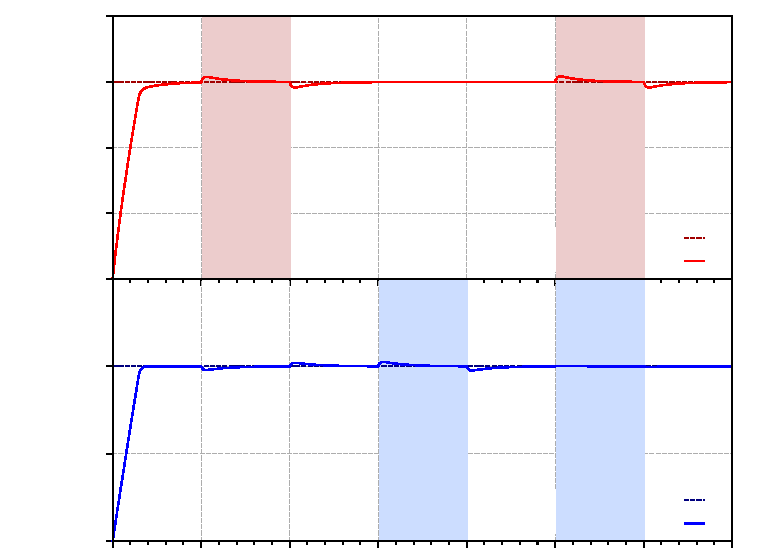
\includegraphics{fsieos}}%
    \gplfronttext
  \end{picture}%
\endgroup
}
        \vspace{0.5cm}
        \caption{T$a_i$OStF simulation -- Where $a_i = a_{\tiny \text{MED}}/4$.}
        \label{fig:fsieos}
    \end{minipage}
    \hfill
    \begin{minipage}[b]{0.48\linewidth}
        \scalebox{0.65}{% GNUPLOT: LaTeX picture with Postscript
\begingroup
  \makeatletter
  \providecommand\color[2][]{%
    \GenericError{(gnuplot) \space\space\space\@spaces}{%
      Package color not loaded in conjunction with
      terminal option `colourtext'%
    }{See the gnuplot documentation for explanation.%
    }{Either use 'blacktext' in gnuplot or load the package
      color.sty in LaTeX.}%
    \renewcommand\color[2][]{}%
  }%
  \providecommand\includegraphics[2][]{%
    \GenericError{(gnuplot) \space\space\space\@spaces}{%
      Package graphicx or graphics not loaded%
    }{See the gnuplot documentation for explanation.%
    }{The gnuplot epslatex terminal needs graphicx.sty or graphics.sty.}%
    \renewcommand\includegraphics[2][]{}%
  }%
  \providecommand\rotatebox[2]{#2}%
  \@ifundefined{ifGPcolor}{%
    \newif\ifGPcolor
    \GPcolortrue
  }{}%
  \@ifundefined{ifGPblacktext}{%
    \newif\ifGPblacktext
    \GPblacktexttrue
  }{}%
  % define a \g@addto@macro without @ in the name:
  \let\gplgaddtomacro\g@addto@macro
  % define empty templates for all commands taking text:
  \gdef\gplbacktext{}%
  \gdef\gplfronttext{}%
  \makeatother
  \ifGPblacktext
    % no textcolor at all
    \def\colorrgb#1{}%
    \def\colorgray#1{}%
  \else
    % gray or color?
    \ifGPcolor
      \def\colorrgb#1{\color[rgb]{#1}}%
      \def\colorgray#1{\color[gray]{#1}}%
      \expandafter\def\csname LTw\endcsname{\color{white}}%
      \expandafter\def\csname LTb\endcsname{\color{black}}%
      \expandafter\def\csname LTa\endcsname{\color{black}}%
      \expandafter\def\csname LT0\endcsname{\color[rgb]{1,0,0}}%
      \expandafter\def\csname LT1\endcsname{\color[rgb]{0,1,0}}%
      \expandafter\def\csname LT2\endcsname{\color[rgb]{0,0,1}}%
      \expandafter\def\csname LT3\endcsname{\color[rgb]{1,0,1}}%
      \expandafter\def\csname LT4\endcsname{\color[rgb]{0,1,1}}%
      \expandafter\def\csname LT5\endcsname{\color[rgb]{1,1,0}}%
      \expandafter\def\csname LT6\endcsname{\color[rgb]{0,0,0}}%
      \expandafter\def\csname LT7\endcsname{\color[rgb]{1,0.3,0}}%
      \expandafter\def\csname LT8\endcsname{\color[rgb]{0.5,0.5,0.5}}%
    \else
      % gray
      \def\colorrgb#1{\color{black}}%
      \def\colorgray#1{\color[gray]{#1}}%
      \expandafter\def\csname LTw\endcsname{\color{white}}%
      \expandafter\def\csname LTb\endcsname{\color{black}}%
      \expandafter\def\csname LTa\endcsname{\color{black}}%
      \expandafter\def\csname LT0\endcsname{\color{black}}%
      \expandafter\def\csname LT1\endcsname{\color{black}}%
      \expandafter\def\csname LT2\endcsname{\color{black}}%
      \expandafter\def\csname LT3\endcsname{\color{black}}%
      \expandafter\def\csname LT4\endcsname{\color{black}}%
      \expandafter\def\csname LT5\endcsname{\color{black}}%
      \expandafter\def\csname LT6\endcsname{\color{black}}%
      \expandafter\def\csname LT7\endcsname{\color{black}}%
      \expandafter\def\csname LT8\endcsname{\color{black}}%
    \fi
  \fi
  \setlength{\unitlength}{0.0500bp}%
  \begin{picture}(7200.00,5040.00)%
    \gplgaddtomacro\gplbacktext{%
      \csname LTb\endcsname%
      \put(726,3150){\makebox(0,0)[r]{\strut{} 5}}%
      \csname LTb\endcsname%
      \put(726,3780){\makebox(0,0)[r]{\strut{} 10}}%
      \csname LTb\endcsname%
      \put(726,4409){\makebox(0,0)[r]{\strut{} 15}}%
      \csname LTb\endcsname%
      \put(726,5039){\makebox(0,0)[r]{\strut{} 20}}%
      \csname LTb\endcsname%
      \put(921,2237){\makebox(0,0){\strut{}}}%
      \csname LTb\endcsname%
      \put(1771,2237){\makebox(0,0){\strut{}}}%
      \csname LTb\endcsname%
      \put(2620,2237){\makebox(0,0){\strut{}}}%
      \csname LTb\endcsname%
      \put(3470,2237){\makebox(0,0){\strut{}}}%
      \csname LTb\endcsname%
      \put(4320,2237){\makebox(0,0){\strut{}}}%
      \csname LTb\endcsname%
      \put(5170,2237){\makebox(0,0){\strut{}}}%
      \csname LTb\endcsname%
      \put(6019,2237){\makebox(0,0){\strut{}}}%
      \csname LTb\endcsname%
      \put(6869,2237){\makebox(0,0){\strut{}}}%
      \put(352,3779){\rotatebox{-270}{\makebox(0,0){\strut{}Nível [cm]}}}%
    }%
    \gplgaddtomacro\gplfronttext{%
      \csname LTb\endcsname%
      \put(6278,2913){\makebox(0,0)[r]{\strut{}Ref. $T_1$}}%
      \csname LTb\endcsname%
      \put(6278,2693){\makebox(0,0)[r]{\strut{}Saída $T_1$}}%
    }%
    \gplgaddtomacro\gplbacktext{%
      \csname LTb\endcsname%
      \put(726,0){\makebox(0,0)[r]{\strut{} 0}}%
      \csname LTb\endcsname%
      \put(726,840){\makebox(0,0)[r]{\strut{} 10}}%
      \csname LTb\endcsname%
      \put(726,1680){\makebox(0,0)[r]{\strut{} 20}}%
      \csname LTb\endcsname%
      \put(726,2520){\makebox(0,0)[r]{\strut{} 30}}%
      \csname LTb\endcsname%
      \put(921,-283){\makebox(0,0){\strut{}0}}%
      \csname LTb\endcsname%
      \put(1771,-283){\makebox(0,0){\strut{}15}}%
      \csname LTb\endcsname%
      \put(2620,-283){\makebox(0,0){\strut{}30}}%
      \csname LTb\endcsname%
      \put(3470,-283){\makebox(0,0){\strut{}45}}%
      \csname LTb\endcsname%
      \put(4320,-283){\makebox(0,0){\strut{}60}}%
      \csname LTb\endcsname%
      \put(5170,-283){\makebox(0,0){\strut{}75}}%
      \csname LTb\endcsname%
      \put(6019,-283){\makebox(0,0){\strut{}90}}%
      \csname LTb\endcsname%
      \put(6869,-283){\makebox(0,0){\strut{}105}}%
      \put(352,1260){\rotatebox{-270}{\makebox(0,0){\strut{}Nível [cm]}}}%
      \put(3895,-613){\makebox(0,0){\strut{}Tempo [s]}}%
    }%
    \gplgaddtomacro\gplfronttext{%
      \csname LTb\endcsname%
      \put(6278,393){\makebox(0,0)[r]{\strut{}Ref. $T_2$}}%
      \csname LTb\endcsname%
      \put(6278,173){\makebox(0,0)[r]{\strut{}Saída $T_2$}}%
    }%
    \gplbacktext
    \put(0,0){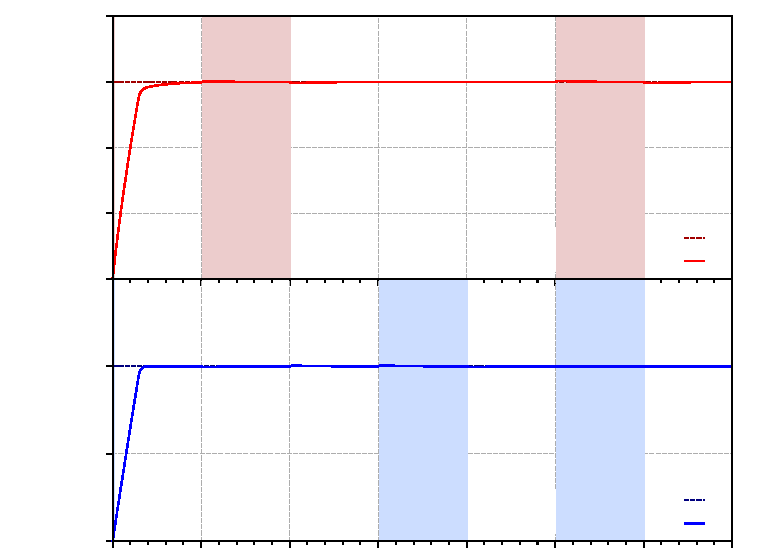
\includegraphics{fsivros}}%
    \gplfronttext
  \end{picture}%
\endgroup
}
        \vspace{0.5cm}
        \caption{T$a_i$VStF simulation -- Where $a_i = a_{\tiny \text{MED}}/2$.}
        \label{fig:fsivros}
    \end{minipage}
\end{figure}

% ==============================================================================
% CONCLUSIONS
% ==============================================================================
\section{CONCLUSIONS}\label{sec:conclusions}
This work was developed in order to provide a FDD system for a coupled water
tanks. For this, the system made use of a neural structure that, from the
processing of the available values, the user was indicated about the faults that
are ocurring.

Since this structure is completely disjointed, another techniques can be mixed
composing a hibrid system for fault detection and diagnosis. The used techniques
can replace those networks whose the performance was below the expectations.

Among the twelve selected faults, eight were easily identified and three had a
satisfactory performance, with a small detection problem that can be solved
through binary flags. The other fault was not correctly identified for $T_2$,
but can be considered reasonable for detection on $T_1$.

The results may improve when the real values are used, since they vary within
the range of values in which the network was trained. This situation can maybe
correct the problem that occurs for detecting UGSeF, UOSeF and TLStF, avoiding
the use of binary flags.

Thus, the system had a satisfactory performance and could be capable to identify
about 92\% of the proposed faults. Proving, therefore, that MLP networks are
efficient structures for identification and for the fault detection and
diagnosis.

Once tested with various excitation signals, the system could be attached to a
FTCS. In this case, the signals generated by the FDD system will serve as an
``alarm''. The FTCS, in turn, may perform the controllers reconfiguration by
modifying their parameters, or even their structures, so that the system
continues to function properly until the fault has been corrected.

% ==============================================================================
% ACKNOWLEDGEMENTS
% ==============================================================================
\section{ACKNOWLEDGEMENTS}
The authors thank CAPES for financial support and also the colleagues in ITA and
UFPA.

% ==============================================================================
% REFERENCES
% ==============================================================================
\section{REFERENCES}

\bibliographystyle{cobem}
\renewcommand{\refname}{}
\bibliography{bibfile}

\end{document}
